%\documentclass{acmsiggraph}              % final
\documentclass[review]{acmsiggraph}       % review
%\documentclass[widereview]{acmsiggraph}  % wide-spaced review
%\documentclass[preprint]{acmsiggraph}    % preprint

%% Uncomment one of the four lines above depending on where your paper is
%% in the conference process. ``review'' and ``widereview'' are for review
%% submission, ``preprint'' is for pre-publication, and ``final'' is for
%% the version to be printed.

%% The 'helvet' and 'times' packages define the typefaces used for
%% serif and sans serif type in this document. Computer Modern Roman
%% is used for mathematics typesetting. The scale factor is set to .92
%% to bring the sans-serif type in line with the serif type.

\usepackage[scaled=.92]{helvet}
\usepackage{times}

%% The 'graphicx' package allows for the inclusion of EPS figures.

\usepackage{graphicx}
\usepackage{amsmath}

%% use this for zero \parindent and non-zero \parskip, intelligently.

\usepackage{parskip}

%% Optional: the 'caption' package provides a nicer-looking replacement
%% for the standard caption environment. With 'labelfont=bf,'textfont=it',
%% caption labels are bold and caption text is italic.

\usepackage[labelfont=bf,textfont=it]{caption}
\usepackage{subfig}

%% If you are submitting a paper to the annual conference, please replace
%% the value ``0'' below with the numeric value of your OnlineID.
%% If you are not submitting this paper to the annual conference,
%% you may safely leave it at ``0'' -- it will not be included in the output.

\onlineid{0241}

%% Paper title.

\title{Lightweight 3D Modeling of Urban Buildings From Range Data}
\author{Weihong Li\thanks{e-mail: wli@gc.cuny.edu}\\ City College of New York / CUNY %
\and George Wolberg\thanks{e-mail: wolberg@cs.ccny.cuny.edu}\\ City College of New York / CUNY %
\and Siavash Zokai\thanks{e-mail: zokai@brainstormllc.com}\\ Brainstorm Technology LLC}

%% Keywords that describe your work.

\keywords{3D modeling, urban buildings, range data, point clouds, geometry compression}

\newcommand{\Eq}[1] {Eq.~(\ref{eq:#1})}
\newcommand{\Fig}[1]{Fig.~\ref{fig:#1}}
\newcommand{\Sec}[1]{Sec.~\ref{sec:#1}}
\newcommand{\Eqs}   {Eqs.~}
\newcommand{\Figs}  {Figs.~}
\newcommand{\Tbl}[1]{Table~\ref{tbl:#1}}
\newcommand{\Etal}  {{\it et al.}}
\newcommand{\Figa}[1]{Fig.~\ref{fig:#1}(a)}
\newcommand{\Figb}[1]{Fig.~\ref{fig:#1}(b)}
\newcommand{\Figc}[1]{Fig.~\ref{fig:#1}(c)}
\newcommand{\Figd}[1]{Fig.~\ref{fig:#1}(d)}

\graphicspath{{figures/}}

%%%%%% START OF THE PAPER %%%%%%

\begin{document}

\teaser{
\begin{center}
\begin{tabular}{cccc}
	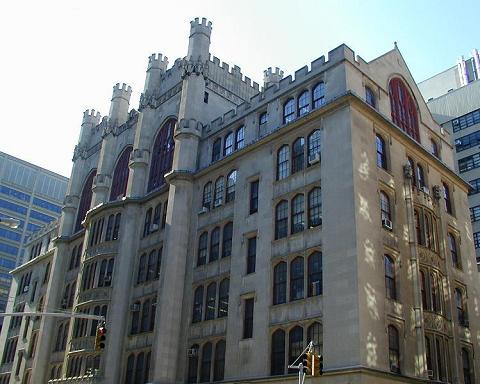
\includegraphics[width=1.5in]{HunterPhoto.jpg} &
	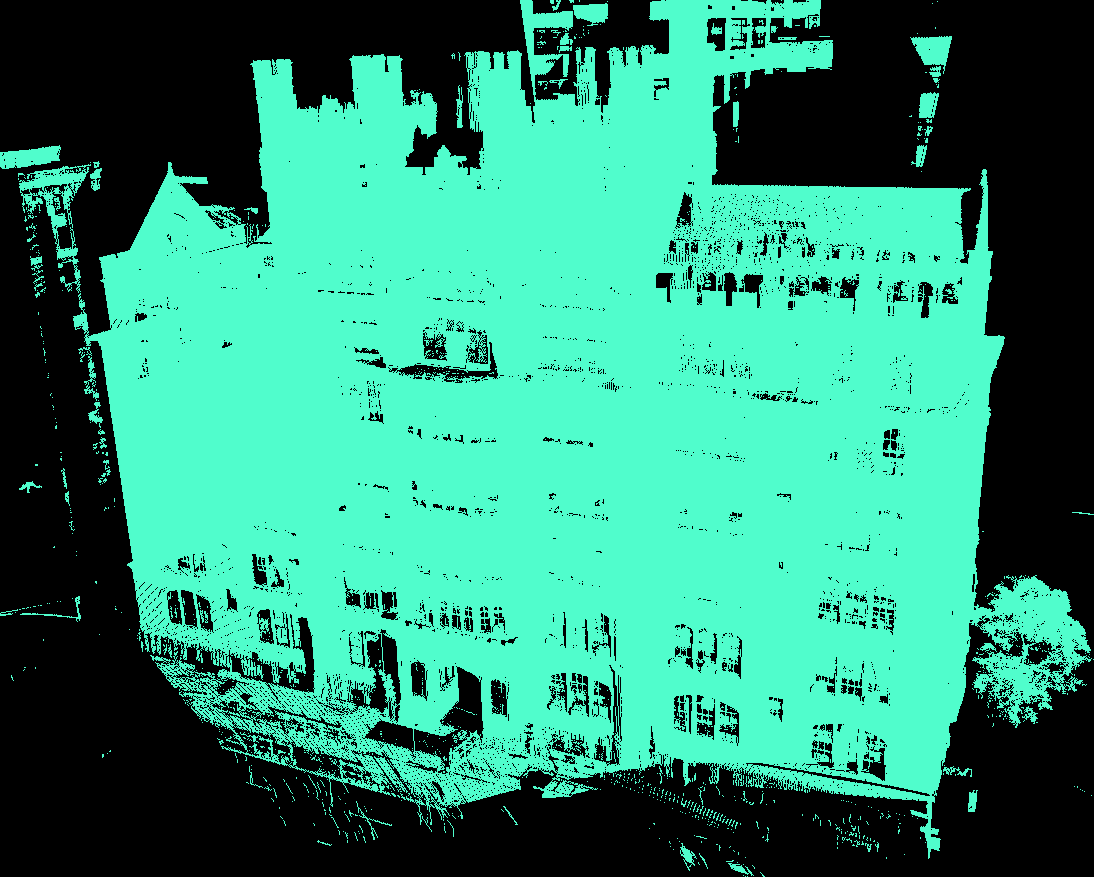
\includegraphics[width=1.5in]{point_cloud.png} &
	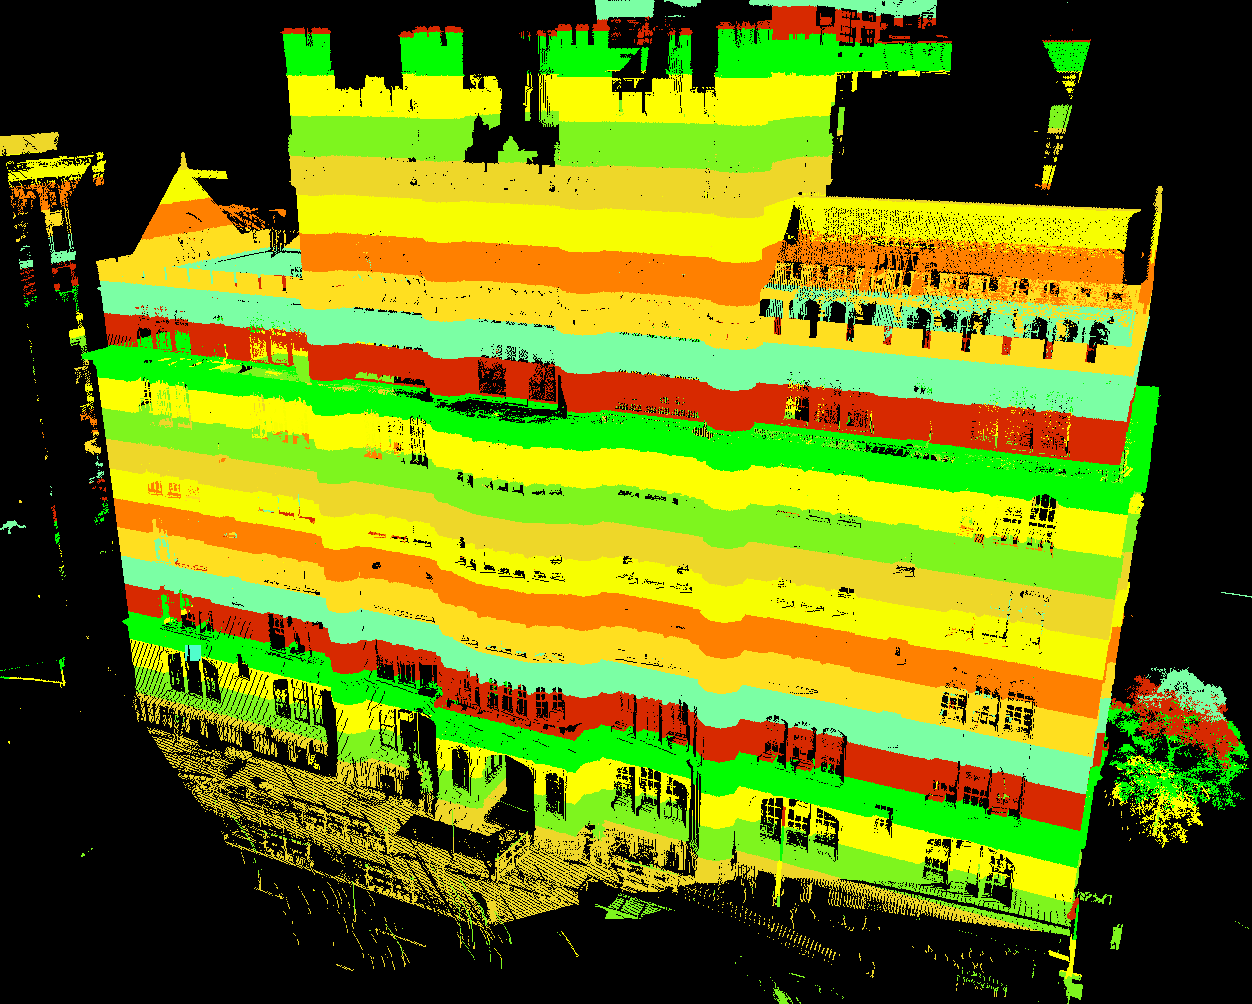
\includegraphics[width=1.5in]{slab_noplanar.png} &
%	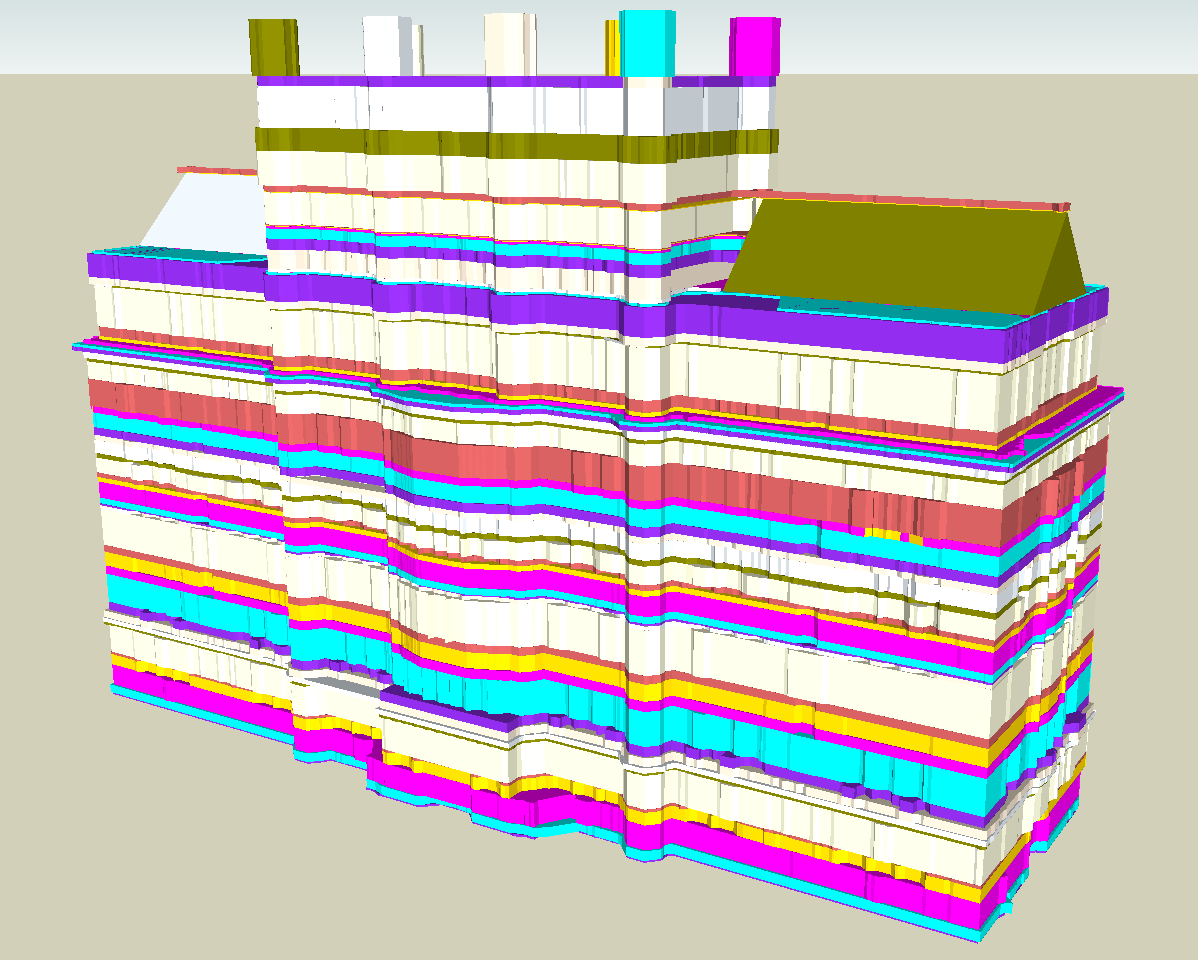
\includegraphics[width=1.5in]{extrusion_1000_4_1.png} &
	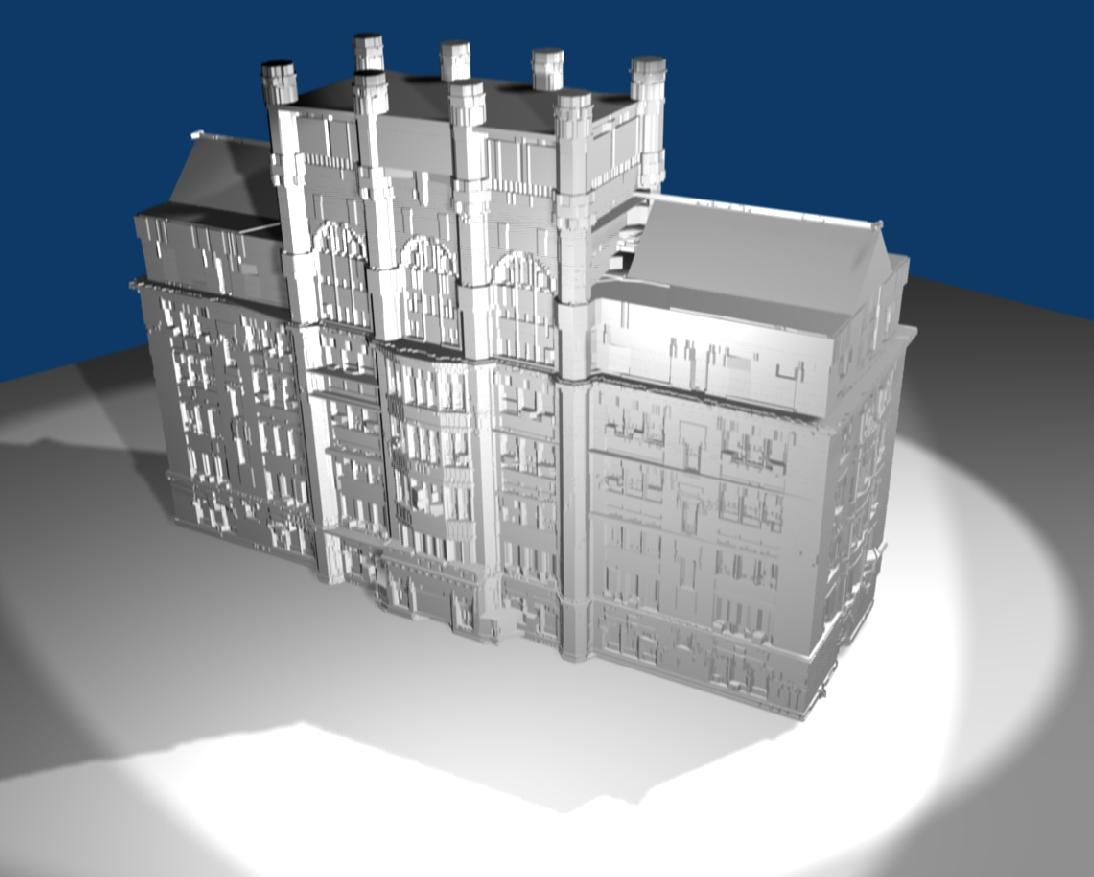
\includegraphics[width=1.5in]{HunterShaded.jpg} \\
	(a) & (b) & (c) & (d) \\
\end{tabular}
\end{center}
\caption{
(a) Image of building to be modeled.
(b) 3D point cloud of building assembled by registering multiple scans.
(c) Slabs of the 3D point cloud data are used to determine prominent
cross-sections upon which extrusion/taper operations are applied.
(d) Rendering of lightweight reconstructed 3D model.
}
\label{fig:IR_2_DXF}
}

%% The ``\maketitle'' command must be the first command after the
%% ``\begin{document}'' command. It prepares and prints the title block.

\maketitle

\begin{abstract}
Laser range scanners are widely used to acquire accurate scene measurements.
The massive point clouds they generate, however, present challenges to
efficient modeling and visualization.
State-of-the-art techniques for generating 3D models from voluminous
range data is well-known to demand large computational and storage requirements.
In this paper, attention is directed to the modeling of urban buildings
directly from range data.
We present an efficient modeling algorithm that exploits \emph{a priori}
knowledge that buildings can be modeled from cross-sectional contours
using extrusion and taper operations.
Inspired by this simple workflow, we identify key cross-sectional slices among
the point cloud.
These slices capture changes across the building facade along the principal axes.
Standard image processing algorithms are used to remove noise, fill holes,
and vectorize the projected points into planar contours.
Applying extrusion and taper operations to these contours
permits us to achieve dramatic geometry compression, making the resulting
models suitable for web-based applications such as Google Earth
or Microsoft Virtual Earth.
This work has applications in architecture, urban design, virtual city
touring, and online gaming.
We present experimental results on the exterior and interior of urban building
datasets to validate the proposed algorithm.
\end{abstract}

\begin{CRcatlist}
\CRcat{I.4.8}{Image Process and Computer Vision}%
{Scene Analysis}{Surface Fitting};
\CRcat{I.3.5}{Computer Graphics}%
{Computational Geometry and Object Modeling}{Modeling Packages}
\end{CRcatlist}

%% The ``\keywordlist'' command prints out the keywords.
\keywordlist


\section{Introduction}
The 3D modeling of urban buildings is an area of active research
with increasing attention drawn from the computer graphics and
computer vision communities.
Current state-of-the-art algorithms include procedural modeling,
3D laser scanning, and image-based approaches.
In addition, conventional modeling tools are commonly used for this purpose.
The most accurate input source for modeling {\it existing} buildings, though,
remains laser range scanners.
They provide high geometric detail by collecting range data from hundreds
of meters away with an accuracy on the order of a few millimeters.
This fidelity is appropriate for construction, architecture, cultural
heritage, and forensics applications.
Unfortunately, laser range scanning can produce an overwhelming amount of data,
which poses great challenges to visualization software that require lightweight
3D models for interactive use.
Polygonal data generated from range scans are therefore too dense for use in
web-based applications such as Google Earth and Microsoft Virtual Earth.
These applications work best with lightweight models consisting of only
hundreds of polygons.

The goal of this work is to automatically produce high-quality
lightweight models of urban buildings from large-scale 3D range data.
The proposed solution is inspired by the simple paradigm embedded in
procedural modeling as well as interactive tools such as Google SketchUp.
The core of these methods is that a simple set of extrusion and taper
operations applied to 2D contours can grow a wide array of complex 3D urban
models.
We propose a reverse engineering approach to infer key cross-sectional
planar contours along with a set of extrusion and taper operations to derive
lightweight models that conform to the 3D range data.

The proposed algorithm can generate models across a wide spectrum of
resolutions.
A particularly useful feature of the algorithm is that it outperforms
existing approximation techniques by preserving the sharpness of the raw
data, even at low resolution.
The contribution of this work is that it combines the benefits of
\emph{a priori} knowledge of urban buildings and fast 2D image
processing techniques to perform 3D modeling of urban buildings directly
from point cloud data.
This offers the benefit of a cost-effective geometry compression
approach for voluminous range data within the domain of urban structures.
It can be applied to boost web-based 3D applications, virtual city touring,
and online gaming.

\section{Related Work}

\begin{figure*}[htbp]
\begin{center}
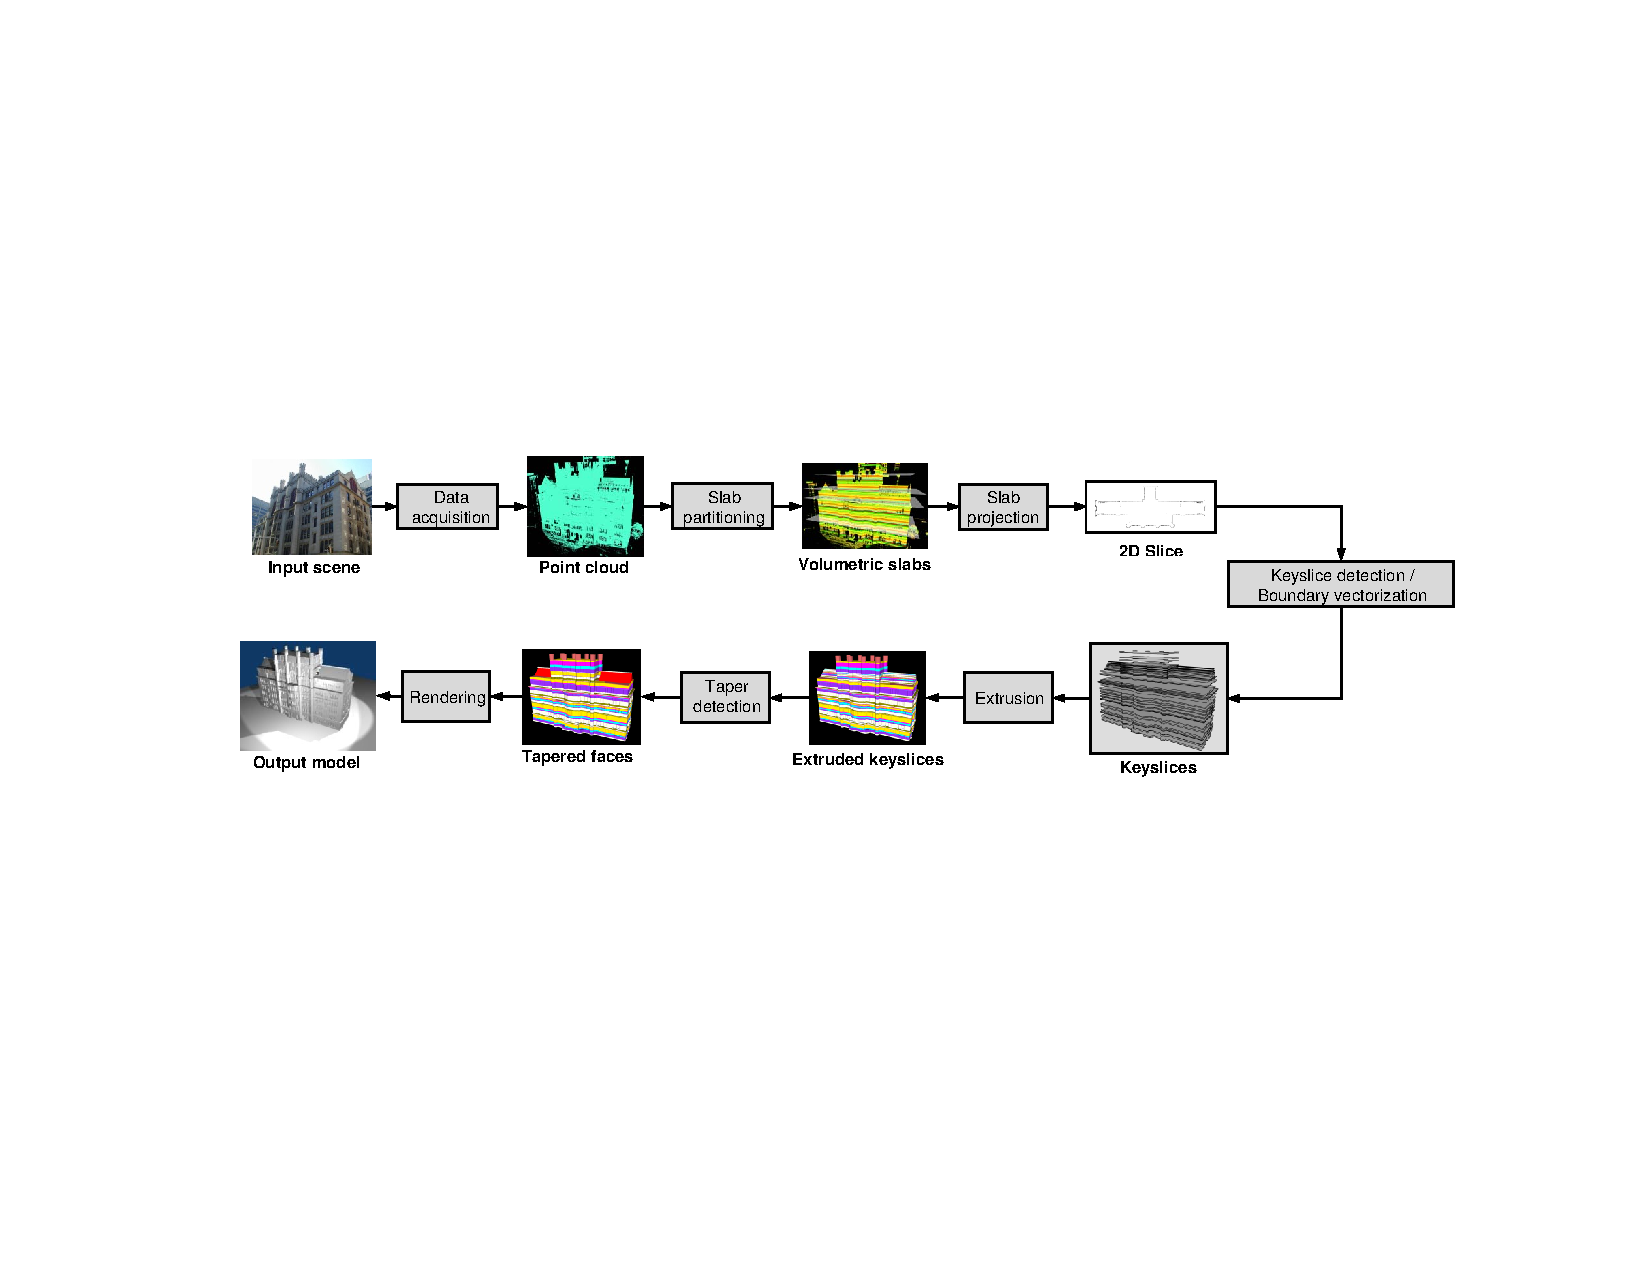
\includegraphics[width=7in]{overview.pdf}
\end{center}
\caption{Overview of the proposed approach.}
\label{fig:ov}
\end{figure*}

In an attempt to steer clear of tedious and expensive hand-made models,
procedural modeling of buildings in \cite{PMB_MWH,PMB_WWS,PMB_PM} has been proposed.
By using an effective description language, buildings and streets of a virtual
city can be generated automatically.
The strength of this approach is that the description language can generate
a huge number of buildings and streets quickly and beautifully.
This is particularly useful for gaming and other computer graphics applications.
However, since the parameters used to generate the buildings are randomly
generated, the city generated with these buildings and streets is a virtual one.
This approach is not useful for attempting to model an {\it existing} building.
In order to do so, one has to manually specify the parameters of the building,
which is very cumbersome.
Our goal is to automatically infer the contours and extrusion/taper parameters
of an existing building directly from dense range data.

Reconstruction of 3D models from range data has been addressed in
\cite{RE_Fisher,RE_CLF,RE_CD} with applications in numerous research areas,
including computer-aided design (CAD), computer vision, architectural modeling,
and medical image processing.
In \cite{DP_OWYC}, the authors proposed a 3D building reconstruction from a
2D floorplan image.
With the help of a 2D floorplan image, both the interior and exterior of a
building can be reconstructed accordingly.
A survey on methods for generating 3D building models from architectural
floor plans is given in \cite{YIN09}.
However, reliance on 2D floor plans makes this approach too limiting for
most applications, including our project.
In \cite{RE_TOGSH}, known manufacturing features were used to infer the
3D structure of mechanical parts.
Their method benefits from the domain knowledge that most of the mechanical
parts consist of predefined structures, such as holes, bosses, and grooves.
Our work is partially motivated by this idea since it also incorporates
{\it a priori} knowledge about the construction of urban buildings for further
inference.
However, their method is based on predefined simple geometry structures and
the assumption that the input 3D data has no holes.
This hinders their approach for those applications with incomplete data.

Multimodal data fusion is another approach for large-scale urban
environment modeling.
In \cite{UM_Zakhor,UM_HYN}, both air and ground data are fused, including
laser scans, camera images, and aerial images.
The LIDAR scans are used to create the models and the camera images are used
for texture mapping.
Citing the cumbersome and expensive use of laser scanners, the researchers
in \cite{AKBARZADEH06} propose an approach that relies solely on passive
sensors (cameras) mounted on a moving vehicle.
Dense 3D point cloud measurements are derived using their multiview stereo
module based on multiple plane sweeping directions.
In an attempt to compress the voluminous data produced in the method of
\cite{AKBARZADEH06}, Xiao et al. \cite{UM_XFTQ} introduced an alternate
approach for modeling facades along a street using prior knowledge about
the buildings.
They achieve geometry compression and deliver a clean approximation of the
facades by applying a combination of plane fitting and window detection.
Their method, however, relies on limited assumptions about the planarity of
the buildings.
The method introduced in this paper, however, places no such limitations.
We can handle facades of any shape that exploit extrusion and taper operations.

The ball-pivoting algorithm (BPA) \cite{BPA_BMRS} is an efficient technique
for meshing 3D point clouds to produce polygonal models.
The generated meshes, however, constitute heavyweight models,
with the number of vertices nearly approaching the number of points in the
3D point cloud.
This limits its usefulness for web-based applications.
Although a BPA model can be simplified using approximation techniques such as
{\it qslim} \cite{BPA_GH}, the sharp detail of the original model is not
preserved.

%%%%%%%%%%%%%%%%%%%%%%%%%%%%%%%%
%%%%%%   Overview  %%%%%%%%
%%%%%%%%%%%%%%%%%%%%%%%%%%%%%%%%
\section{Overview}

We propose an efficient way to reconstruct 3D models from range data by
partitioning the data into thin cross-sectional volumetric slabs.
For each slab, all range data in that slab is projected onto a 2D
cross-sectional contour slice.
Producing this array of slices permits us to avoid costly computation directly
on 3D data.
A similarity measure \cite{IR_Brown} is used to cluster the sliced images
together into {\it keyslices}.
This term is analogous to the use of ``keyframes'' in computer animation,
which denote important snapshots in the animation sequence from which
intermediate results can be derived.
In essence, each keyframe is a slice in the spatiotemporal volume of
an animation.
Similarly, each keyslice is a 2D image which contains a {\it transitional}
cross-section of the building, encapsulating major contours in the facade.
The model is then generated by applying basic extrusion and taper
operations from one keyslice to the next.
This produces a lightweight representation consisting of only a few
hundred polygons.

An overview of our approach, depicted in \Fig{ov}, begins with the
acquisition of a dense 3D point cloud $C$ of a building.
$C$ is then partitioned into a nonoverlapping set of volumetric slabs.
Each slab $S$ is associated with one projection plane $P$,
sitting at the base of $S$.
The purpose of partitioning $C$ is to establish a set of cross-sections,
or contour slices.
By examining the changes among these slices, we can identify the prominent
slices, or {\it keyslices}, as well as the necessary extrusion and
taper operations that must apply to them to generate the model.
By casting this 3D modeling task into a series of 2D operations, we
reduce the dimension of the problem to achieve a significant savings in
computational complexity.

Due to occlusion and material-dependent reflection problems off of glass
(e.g., windows), the input data is incomplete and noisy.
Therefore, noise removal and hole filling are carried out as a
preprocessing stage to generate the 3D model.
The next stage of the approach is to carry out fast image processing
techniques on the enhanced image slices to detect keyslices.
Boundary vectorization for these raster keyslices is then conducted to
transform these points into polygons.
Tapered structure detection is carried out to further reduce the model size.
Finally, 3D model generation is achieved by applying the extrusion/taper
operations to the keyslices to reconstruct lightweight 3D models of urban
buildings from range data.

%%%%%%%%%%%%%%%%%%%%%%%%%%%%%%%%
%%%%%%   PREPROCESSING  %%%%%%%%
%%%%%%%%%%%%%%%%%%%%%%%%%%%%%%%%
\section{Preprocessing the Range Data}
\label{sec:prep}

The input to our system is range data assembled as a 3D point cloud.
Our data is obtained from a Leica Cyrax 2500 laser range scanner \cite{RDP_LRS},
which works by sweeping an eye-safe laser beam across the scene to collect
up to one million 3D depth points per frame.
All scene points that lie within 100 meters can be acquired with an accuracy
of 5mm in depth.
The basic algorithm that we use for registering the voluminous 3D data
acquired from multiple scans of buildings has been introduced in
\cite{RDP_LS}.
That same algorithm is also responsible for extracting the major axes
of the building in order to align it to the axes of the world coordinate
system.
This is necessary to properly infer the keyslices.
\Figb{IR_2_DXF} displays a properly aligned, {\it registered} 3D point cloud
consisting of 14 scans totalling 14 million points.

Due to occlusions and limited vantage points, the point cloud collected by the
laser scanner contains artifacts and holes.
In addition, computing directly on 3D data is time-consuming and
computationally complex.
To tackle these issues, we define inner and outer bounding boxes for the
building to clip away unrelated scene objects.
Then, we convert the 3D modeling problem into a set of 2D problems by
projecting the 3D data into a series of 2D cross-sectional contour images.
Noise removal, hole filling, and vectorization are all done in this
2D space.

\subsection{Extraction of 2D Slices}
\label{sec:image_slicing}

We consider the point cloud data as a large array of 3D points to be
sliced into horizontal volumetric slabs.
All 3D points within each slab are projected onto a horizontal projection
plane, or slice, at the base of the slab.
\Fig{slice_slab} shows the 3D point cloud in \Figb{IR_2_DXF} partitioned into
50 slabs.
The 3D points in each slab are projected onto a projection plane to
form cross-sectional contour slices.
\Fig{slicing} depicts four such slices, associated with the four displayed
projection planes of \Fig{slice_slab}.

\begin{figure} [htbp]
\begin{center}
\begin{tabular}{cc}
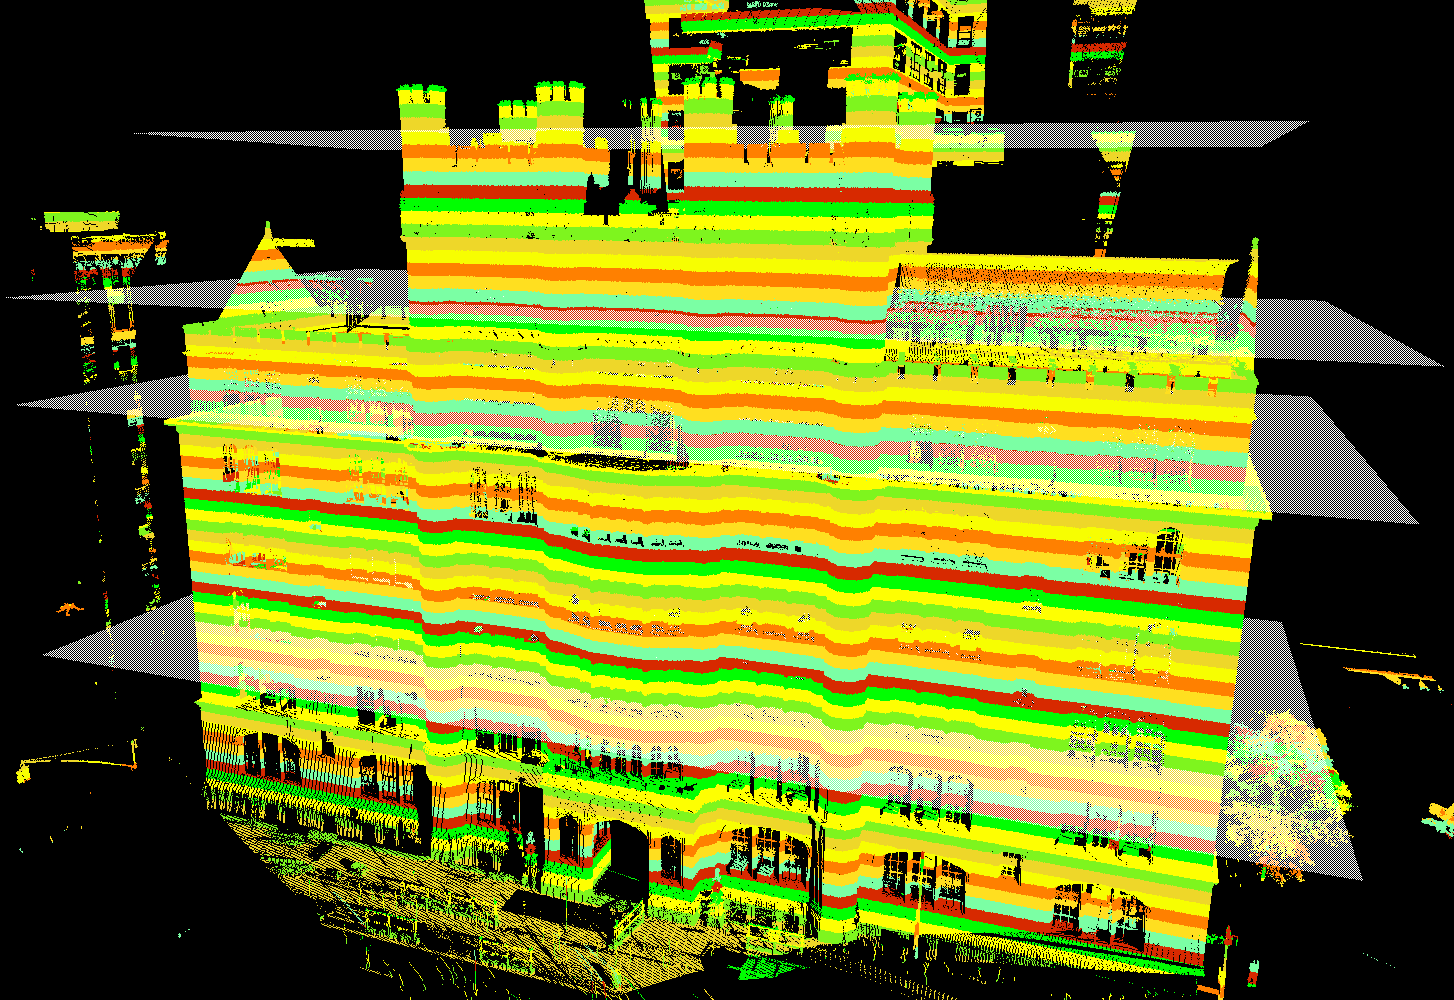
\includegraphics[width=0.3\textwidth]{slab_planar.png}
\end{tabular}
\end{center}
\caption{The 3D point cloud of \Figb{IR_2_DXF} partitioned into uniform
volumetric slabs.
The 3D points in each slab are projected onto a projection plane to
form cross-sectional slices. Four such planes are shown.}
\label{fig:slice_slab}
\end{figure}

The height of each slab is $\boldsymbol{\delta}$.
If $\boldsymbol{\delta}$ is held constant, each slice is generated from
equi-spaced slab intervals.
If $\boldsymbol{\delta}$ is allowed to vary, then we may
choose to allow for large values in parts of the structure that are similar,
and low values in regions that contain finer detail.
To avoid working on 3D data directly, a relatively small constant value
for $\boldsymbol{\delta}$ is chosen to generate 2D cross-sectional image slices.

\begin{figure} [htbp]
\begin{center}
\begin{tabular}{cc}
\fbox{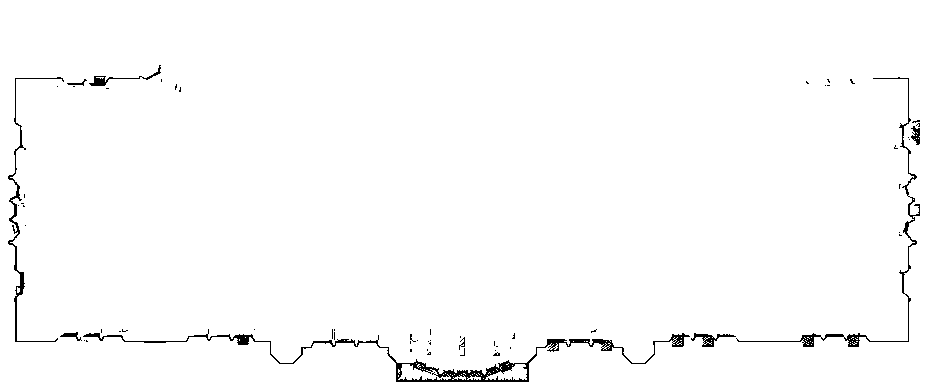
\includegraphics[width=0.2\textwidth]{image_slice_0190.png}} &
\fbox{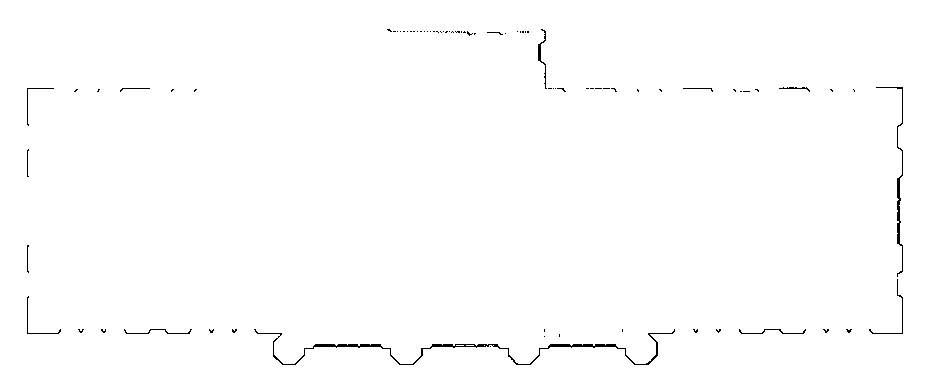
\includegraphics[width=0.2\textwidth]{image_slice_0600.png}} \\
(a) & (b) \\
\fbox{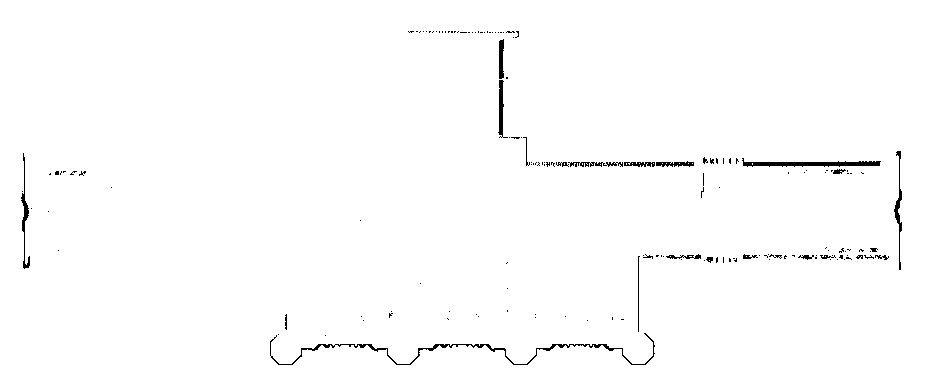
\includegraphics[width=0.2\textwidth]{image_slice_0714.png}} &
\fbox{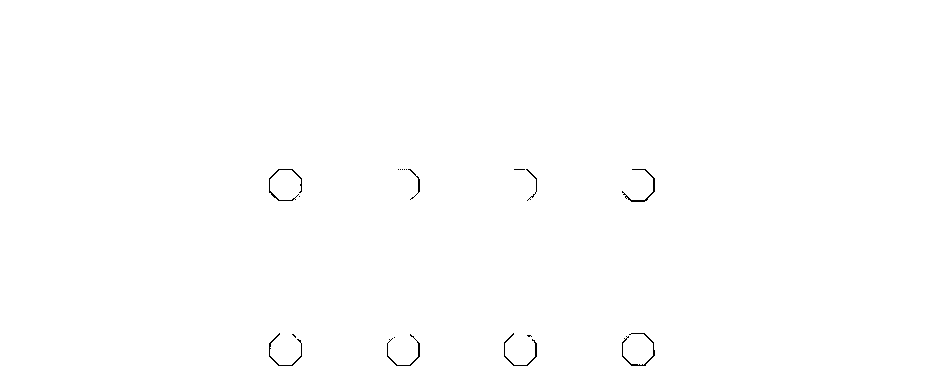
\includegraphics[width=0.2\textwidth]{image_slice_0951.png}} \\
(c) & (d)
\end{tabular}
\end{center}
\caption{The set of slices corresponding to the four projection planes in
\Fig{slice_slab}.}
\label{fig:slicing}
\end{figure}

Without loss of generality, the $y-$axis is used to represent the bottom-up
vertical direction.
Over each slab in height range $[H_{lo}, H_{hi})$,
we project the 3D data $\boldsymbol{P}(x,y,z)$, for $H_{lo} \leq y < H_{hi}$,
onto a 2D image slice.
The projection is normalized in the range $[0,W]$, where $W$ is the image width:
\begin{equation}
[\,x^{2D},\; y^{2D}\,]^T = \omega\cdot[\,x^{3D}_i - X_{MIN},\; z^{3D}_i - Z_{MIN}\,]^T
\label{eq:image_slicing}
\end{equation}
Note that $\omega = W/(X_{MAX} - X_{MIN})$, and that
the [$X_{MIN}$, $X_{MAX}$] and [$Z_{MIN}$, $Z_{MAX}$] pairs define the
3D bounding box, which can be obtained through user input and can be used
to clip away noise data.
\Fig{slicing}(a)-(d) show some examples of the 2D slices, where noise
and incomplete data are observed.

\subsection{Hole Filling}
\label{sec:mdr}

The slices we extract above often have holes (i.e., missing data) due to
occlusion or other visibility issues.
Fortunately, most urban buildings have symmetry that we can exploit to
fill these holes.
Symmetry computation on 3D data \cite{Sym_PSGRF,Sym_ZPA} is expensive,
so we conduct this computation on the 2D image slices.
Since the 3D data has been already rectified \cite{RDP_LSYGS} and projected onto 2D slices, hence only 2D translation
is needed to be considered for symmetry computation.
Let $P(x,y)$ be a point on the original image $I$ and $P'(x',y')$ be the reflected
point of $P$ with respect to a symmetry line $L$.
The symmetry computation equation for $L$ is as follows:
\begin{equation}
L = \underset{x,y}{\operatorname{arg\,min}}\sum{d_{x,y}(P', I)}
\end{equation}
where the $d_{x,y}(P',I)$ is the distance between the self-reflected point
$P'$ and its nearest data point in image $I$.
The reflected point $P'$ of the original point $P$ is computed with
respect to a line along either the $x-$ or $y-$ axis.
Therefore, the symmetry line $L$ is obtained as the line with minimum
summation error over the reflected data points.
\Figa{sym} and \Figb{sym} depict the original input with holes, and
the output after hole filling using symmetry computation, respectively.

\begin{figure}[htbp]
\begin{center}
\begin{tabular}{cc}
\fbox{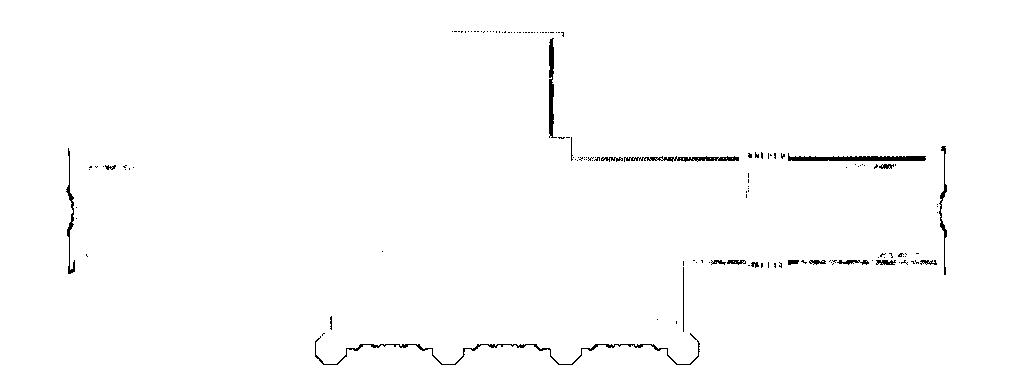
\includegraphics[width=0.2\textwidth]{image_slice_0705_0711.png}} &
\fbox{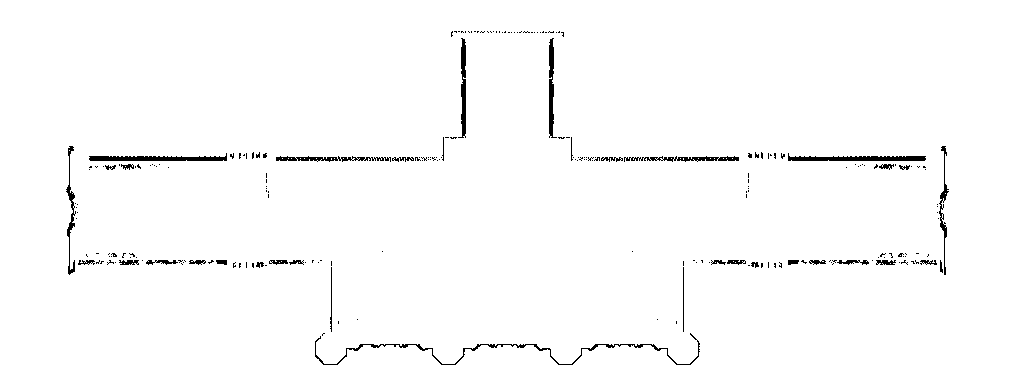
\includegraphics[width=0.2\textwidth]{image_slice_0705_0711_recoverd.png}} \\
(a) & (b)
\end{tabular}
\end{center}
\caption{ Symmetry-based hole filling. (a) Original 2D slice image and
(b) output image after hole filling.}
\label{fig:sym}
\end{figure}

%%%%%%%%%%%%%%%%%%%%%%%%%%%%%%%%
%%%%%%   3D Reconstruction  %%%%
%%%%%%%%%%%%%%%%%%%%%%%%%%%%%%%%
\section{Lightweight 3D Reconstruction}
\label{sec:reconst}
Our 3D modeling algorithm is based on \emph{a priori} knowledge that
urban buildings can be created through a series of extrusion and taper
operations on the salient cross-sections contained in the keyslices.
\Fig{keyslices} depicts the keyslices derived from the uniform slices
given in \Fig{slice_slab}. 
The key step for successful modeling is identifying these salient cross
sections upon which the extrusion and taper operations will apply.

\begin{figure}[hbtp]
\centering
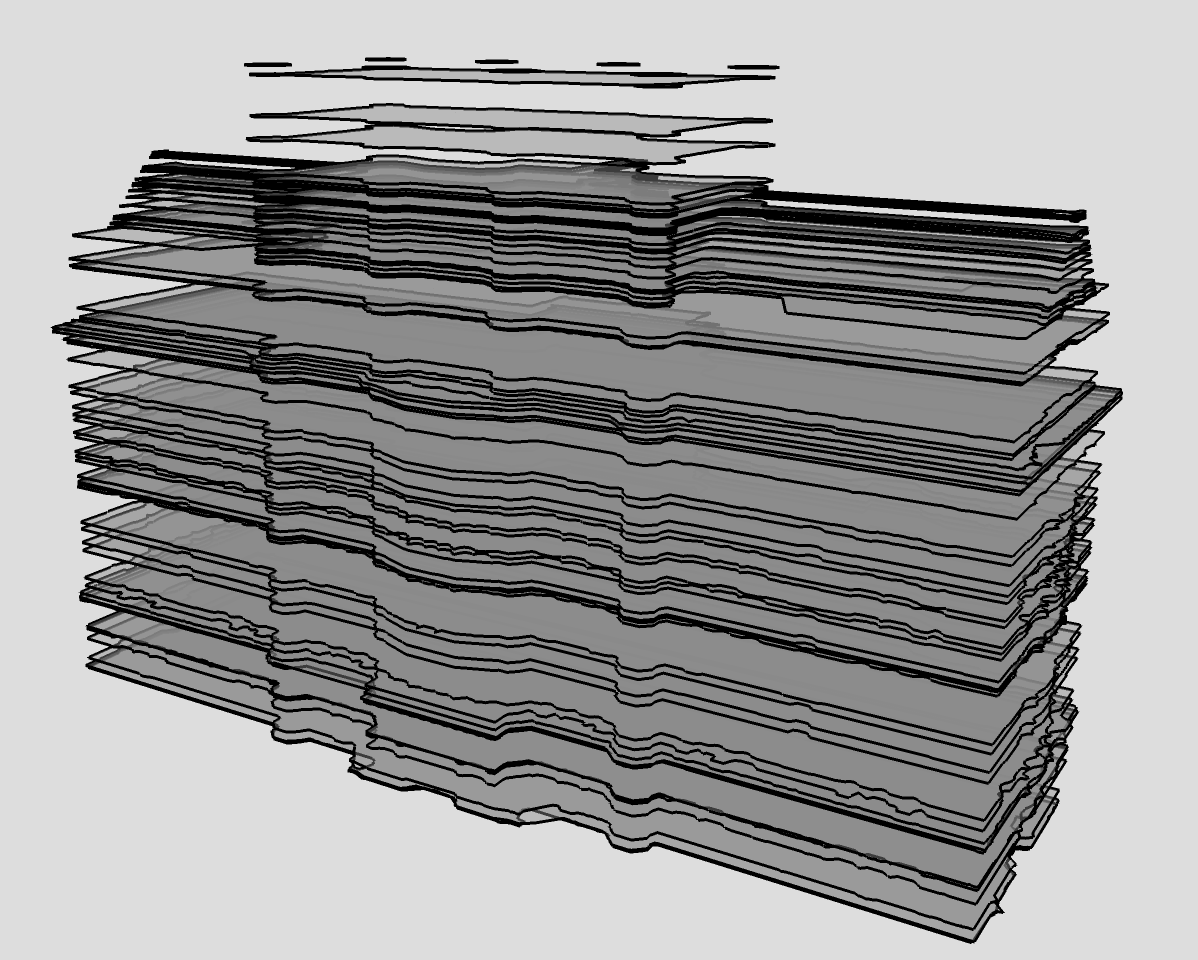
\includegraphics[width=0.35\textwidth]{figures/keyslice_wireframe.png}
\caption{Keyslices derived from the input in \Fig{slice_slab}.}
\label{fig:keyslices}
\end{figure}

\subsection{Keyslice Detection}
\label{sec:ksd}
The 2D image slices of an extruded region are similar to each other.
Thus, to detect the keyslices that delimit extruded regions one only needs
to compute the similarity between adjacent slices.
We select the Hausdorff distance as the similarity measure.
Let $P_r(x_r, y_r)$ be a data point in a reference image and
let $P_i(x_i, y_i)$ be a data point in a new observed image $I$.
The Hausdorff distance of image $I$ to reference image $I_r$ is defined as:

\begin{equation}
d_H(I, I_r) = \sum_{i=0}^Nd_{min}(P_i, I_r)
\label{eq:hd}
\end{equation}

where $d_{min}(P_i, I_r)$ is the minimum distance from data point $P_i$
in image $I$ to the reference image $I_r$.
Alternatively, we can also define the Hausdorff distance, $d_H(I_r, I)$,
from reference image $I_r$ to a new observed image $I$, using \Eq{hd}.
These two distances are usually not equal to each other.
As a rule of thumb, one can choose
$d_{HD} = \text{MAX}\{d_H(I, I_r), d_H(I_r, I)\}$ as the Hausdorff distance.
To compute the keyslices, a threshold $\tau_{d}$ is used for the
Hausdorff distance $d_{HD}$.
If $d_{HD} < \tau_{d}$, the two images $I$ and $I_r$ are considered
similar to each other.
Otherwise, a keyslice image is found and $I_r$ is updated with $I$,
the new keyslice image.

The accuracy of the keyslices detected by using the Hausdorff distance
is closely tied to threshold $\tau_d$.
Small $\tau_d$ leads to more accurate models and will require more time and
space to compute and store the result.
When the threshold $\tau_d$ is relatively large, potential keyslices which
contain salient structure may be missed.
Therefore, there is a trade-off between model accuracy and time-space
efficiency.
To address this problem, the curvature information is computed as a
complementary criteria for keyslice detection.

This idea is based on the observation that the keyslices are generally
located at large curvature changes along 2D slices extracted in the orthogonal
direction (e.g., side view), as shown in \Figa{HT_BPA_Curvature}.
Therefore, instead of computing the difference between two images directly,
we compute the curvature of orthogonal 2D slices, map the positions of
curvature extrema back to cross-sections in the original set of volumetric
slabs, and mark these cross-sections as keyslices.

\begin{figure}[htbp]
\begin{center}
\begin{tabular}{cc}
\fbox{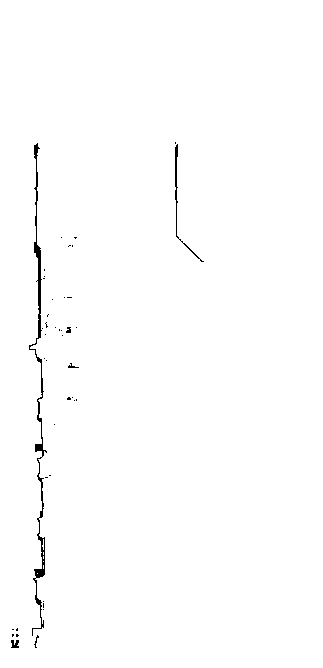
\includegraphics[width=0.1\textwidth]{image_slice_lr_0580_0590_half.png}}
\fbox{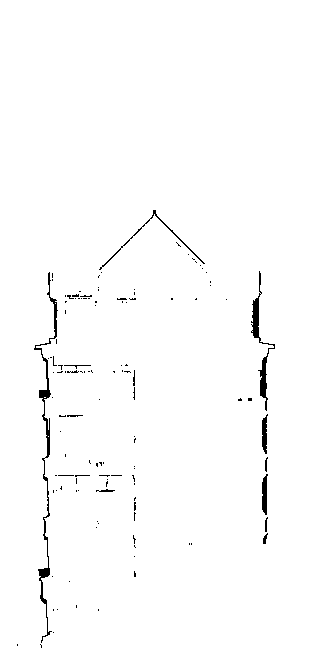
\includegraphics[width=0.1\textwidth]{image_slice_lr_0830_0842_half.png}} &
\fbox{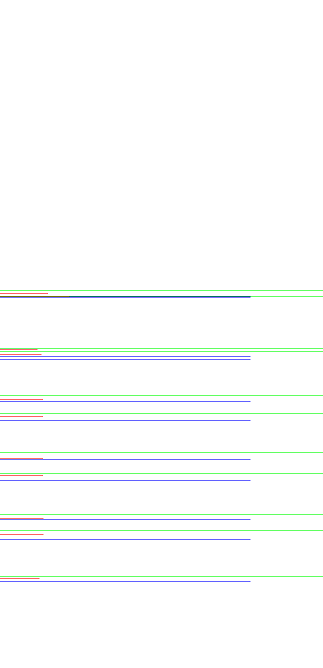
\includegraphics[width=0.1\textwidth]{curvature_center_lines_old_half.png}} \\
(a) & (b)
\end{tabular}
\end{center}
\caption{Curvature-based key slice detection.
(a) A partial set of two 2D sliced images from the orthogonal direction (side
view). The complete set will be used to extract the keyslices shown in
\Fig{keyslices}.
(b) The average curvatures detected over all of the sliced images along the
orthogonal direction.}
\label{fig:HT_BPA_Curvature}
\end{figure}

To compute the curvature, we first apply the slice extraction algorithm
described in \Sec{image_slicing} to obtain a series of 2D cross-sectional
images in the orthogonal direction.
We then apply the ball-pivot algorithm described in \Sec{BPA} to
vectorize the boundary for each sliced image.
We locate those curvatures that appear in most of the sliced images as the
places where keyslices are found, as shown in \Figb{HT_BPA_Curvature}.
Note that the red lines indicate location of the center of the curvature,
and the blue and green lines indicate the entering and exiting of the
curvature structures, respectively.
The combination of Hausdorff distance measurement and curvature inference
ensures that the salient structures of a building will be preserved.

\subsection{Boundary Vectorization}
\label{sec:BPA}

After the keyslices are detected, $N_K$ keyslices will be identified
from a total of $N_A$ image slices.
Depending on the threshold $\tau_{d}$, $N_K$ is usually about one to two
orders of magnitude smaller than $N_A$, e.g., $N_K/N_A$ is 0.06 when
$\tau_d$ = 4.0 for the example in \Figb{IR_2_DXF}.
To generate the 3D model, these keyslice images need to be vectorized to
represent the contours of the building facade.
Several raster image vectorization approaches are proposed in
\cite{DP_AAKMT,DP_DP}.
The Douglas-Peucker algorithm attempts to connect all of the existing points
to form a polygon.
Although the implementation of this approach is very efficient with the
improvement described in \cite{DP_HS}, this method cannot handle the case
where spurious interior points are present, which contributes to outlier data.
To tackle this issue, we adapted the ball-pivoting algorithm (BPA)
\cite{BPA_BMRS} from its original use on 3D point cloud data to use on
2D keyslice images where it produces vectorized boundaries.
The key parameter for the BPA algorithm to work successfully is to
find the right size of the ball for pivoting.
We propose a coarse-to-fine adaptive BPA algorithm, described below,
to solve this problem.

\begin{figure}[hbtp]
\centering
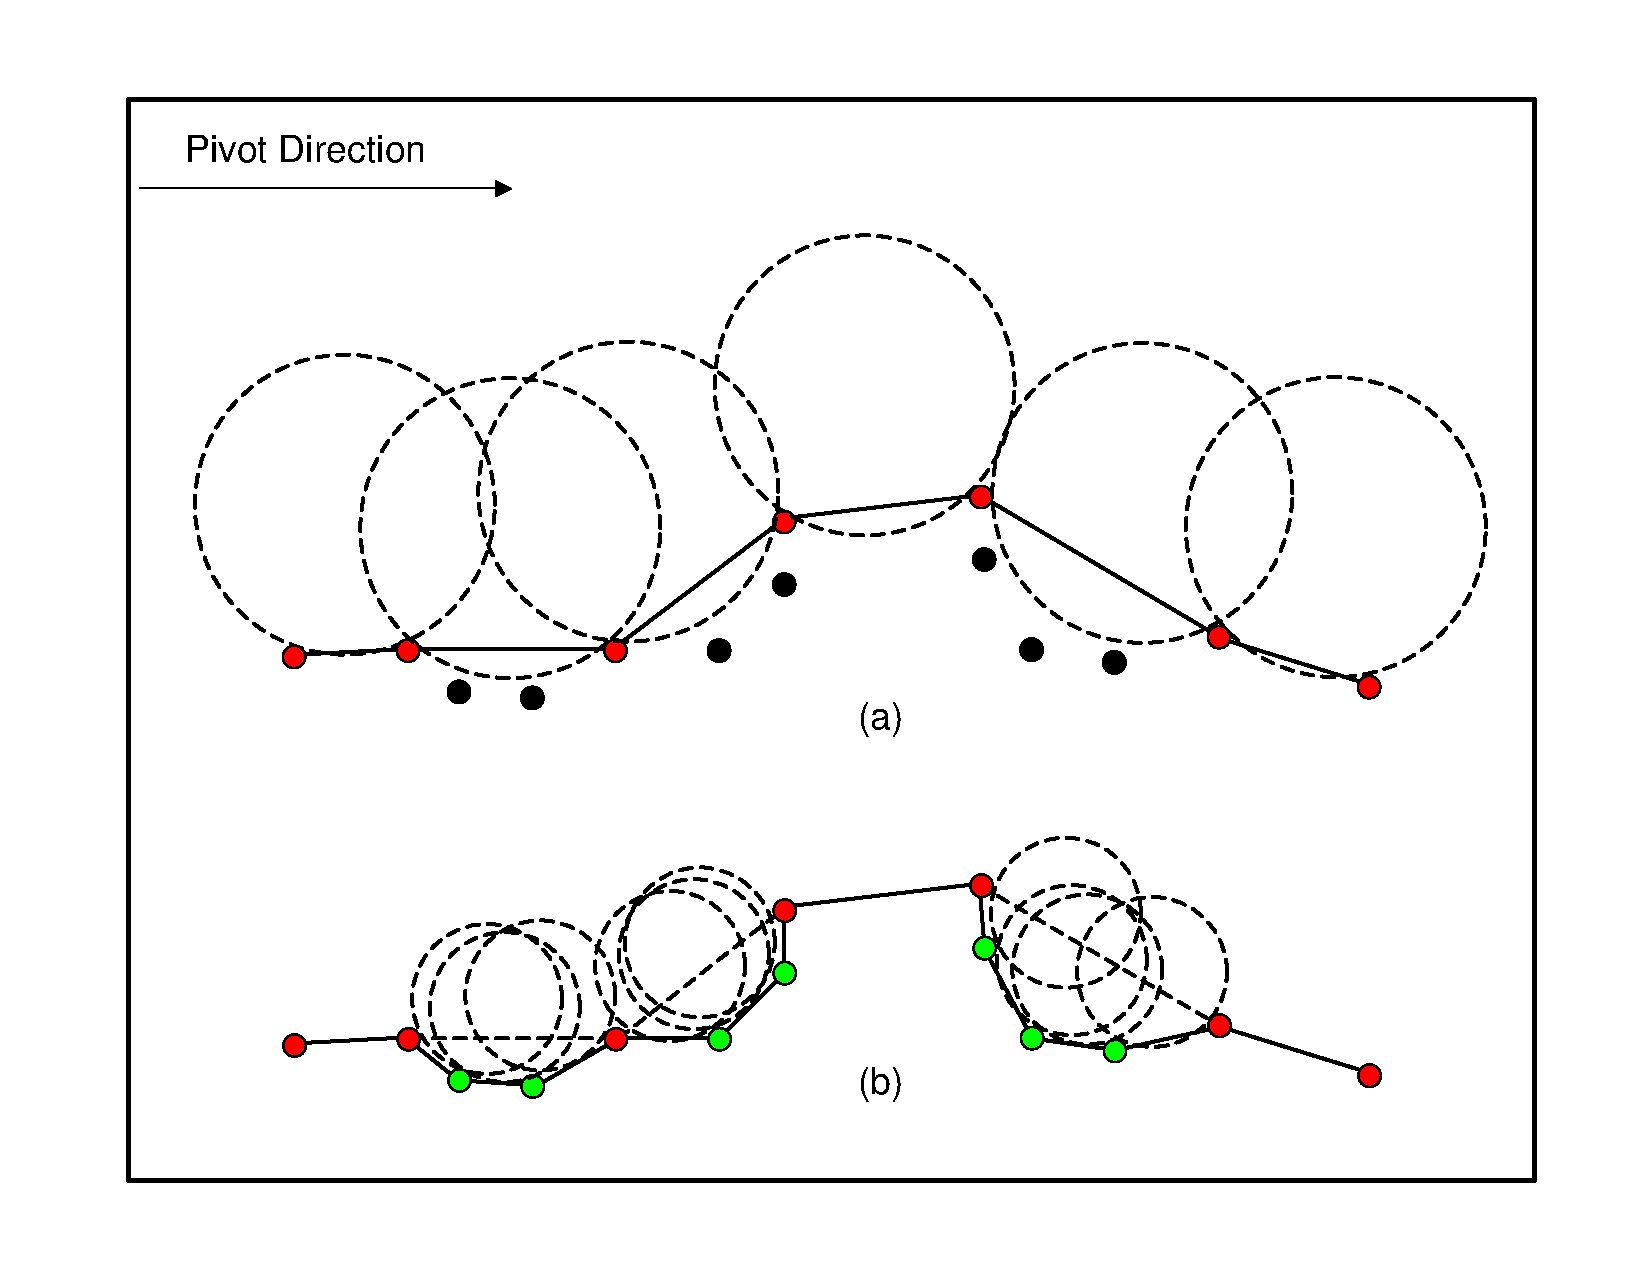
\includegraphics[width=0.4\textwidth]{figures/BPA.pdf}
\caption{Adaptive ball pivoting algorithm:
(a) Initial pivoting with circle of radius 2$r$;
(b) Refinement with circle of radius $r$.}
\label{fig:BPA}
\end{figure}

Due to the gap between data points, a relatively large radius $r$ is chosen
as a coarse step to ensure that the ball will travel across all boundary
data before turning back or reaching any existing boundary points.
\Figa{BPA} shows an initial ball-pivoting process on 2D data points.
The output of the initial BPA $\boldsymbol{\Phi}$ contains an ordered list of the boundary data
points $\boldsymbol{P}$ and their corresponding directions $\overrightarrow{\boldsymbol{R}}$ in which
the circle $C$ starts pivoting.
The iterative BPA refinement process applies a smaller radius $r' = r/2$
to $\boldsymbol{\Phi}$ to get more accurate results, as shown in \Figb{BPA}.
The length of each line segment formed by adjacent points is checked,
$\ell = \overline{P_0P_1}$, in $\boldsymbol{\Phi}$.
If this line is long enough, the BPA is applied between the two adjacent points.
When the ball reaches the second point, a new list of ordered boundary points,
$\boldsymbol{\Phi'}$, is inserted into $\boldsymbol{\Phi}$ between $P_0$ and
$P_1$.
This process continues until it finishes checking every adjacent point in $\boldsymbol{\Phi}$.
The refinement stops when $r'$ falls below threshold $\tau_r$.

%%% Adaptive BPA + HT %%%%

Although the adaptive BPA is a very efficient and straightforward approach to
vectorize the contours of the building facade in the keyslice images,
it produces many short line segments and is sensitive to noise, as shown
in the upper part of the vectorized image in \Figa{HT_BPA_figure}.
Based on the observation that the boundaries of man-made buildings are replete
with lines, we can improve the adaptive BPA results by line fitting using the
Hough transform (HT).

\begin{figure}[htbp]
\begin{center}
\begin{tabular}{c}
\fbox{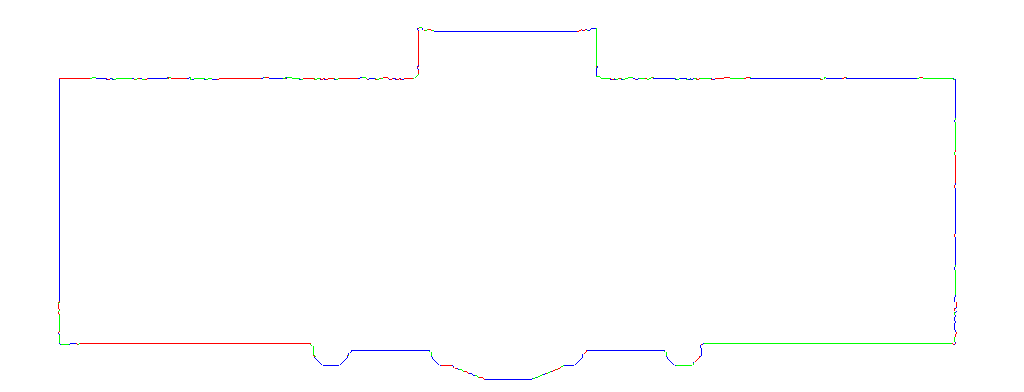
\includegraphics[width=0.35\textwidth]{bbb_image_slice_1024_392_0533_refine_with_rad_1_and_merged.png}} \\
(a) \\
\fbox{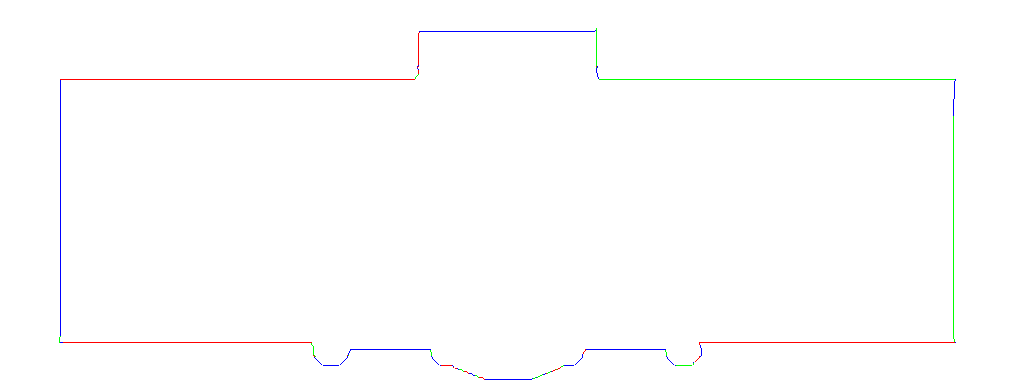
\includegraphics[width=0.35\textwidth]{bbb_image_slice_1024_392_0533_combine_HT_BPA_rad_32.png}} \\
(b)
\end{tabular}
\end{center}
\caption{Boundary vectorization of keyslice image with (a) adaptive BPA
and (b) adaptive BPA / Hough transform.}
\label{fig:HT_BPA_figure}
\end{figure}

To combine the adaptive BPA with HT, we first apply the HT algorithm on the
keyslice image to obtain all lines $\boldsymbol{L}$ and sort them by length. 
The longer lines give more confidence to the line structure of the building.
We integrate the BPA and HT methods by first applying a dilation operation on
$I$ using 8-connected neighbors to get the dilation image, $I_d$.
The next step is to measure how well the lines in $\boldsymbol{L}$ match the
data in $I_d$, which determines whether a line in $\boldsymbol{L}$
should be used as a substitution or not.

If a line segment $L$ is found to be a good candidate, the next step is to
find the corresponding part of the BPA points in $\boldsymbol{\Phi}$ for
substitution. To do this, we first compute the closest two points
$P_i$ and $P_j$ in $\boldsymbol{\Phi}$ to the two end points of $L$.
The points in $\boldsymbol{\Phi}$ represent a polygon and therefore form
a circle layout, i.e., $\boldsymbol{P} = \{ P_0,P_1,\ldots ,P_{n-1}, P_0 \}$.
Assuming $i < j$, there are two possible choices to replace
the series of the points, which are
$\boldsymbol{P_1} = \{ P_i,P_{i+1},\ldots,P_{j-1}, P_j \}$, and
$\boldsymbol{P_2} = \{ P_j,P_{j+1},\ldots,P_{i-1}, P_i \}$.
To determine which one is correct, one can compare the distance, $D$,
from the line $L$ to both set of the points $\boldsymbol{P_1}$ and
$\boldsymbol{P_2}$.
The point set with smaller $D$ is about to be substituted by the line $L$.
\begin{equation*}
D = \underset{\boldsymbol{P_1},\boldsymbol{P_2}}{\operatorname{arg\,min}}\sum{\lVert P_i - L \rVert}
\qquad P_i \in \boldsymbol{P_1} \ \text{or} \ P_i \in \boldsymbol{P_2}
\end{equation*}
where $\lVert P_i - L \rVert$ is the Euclidean distance from point $P_i$ to
line $L$.

After being replaced with line structures detected by the Hough transform,
the beautified contour is shown in \Figb{HT_BPA_figure}.
Notice that the top part of the contour, which consisted of short line
segments, was refined with two long line segments.
This reduces the noise, simplifies the contour, and produces clean models.

\subsection{Tapered Structure Detection}
\label{sec:tsd}

After the keyslices are detected and vectorized, the contours of
$N_K = \{I_{i}, i = 0, ..., K \}$ keyslices are used to represent
the building based on the extrusion operation.
That is, the space between each pair of keyslices, say $I_{i}$ and $I_{j}$,
can be interpolated by the lower keyslice, e.g., $I_{i}$ in this case.
This is valid due to the similarity between the intermediate slices
and the keyslice $I_{i}$.
By modeling a building using this series of keyslices $N_K$, we
significantly reduce the polygon count for urban buildings.
This helps make possible 3D web-based applications such as 3D city navigation.

\begin{figure}[htbp]
\begin{center}
\begin{tabular}{c}
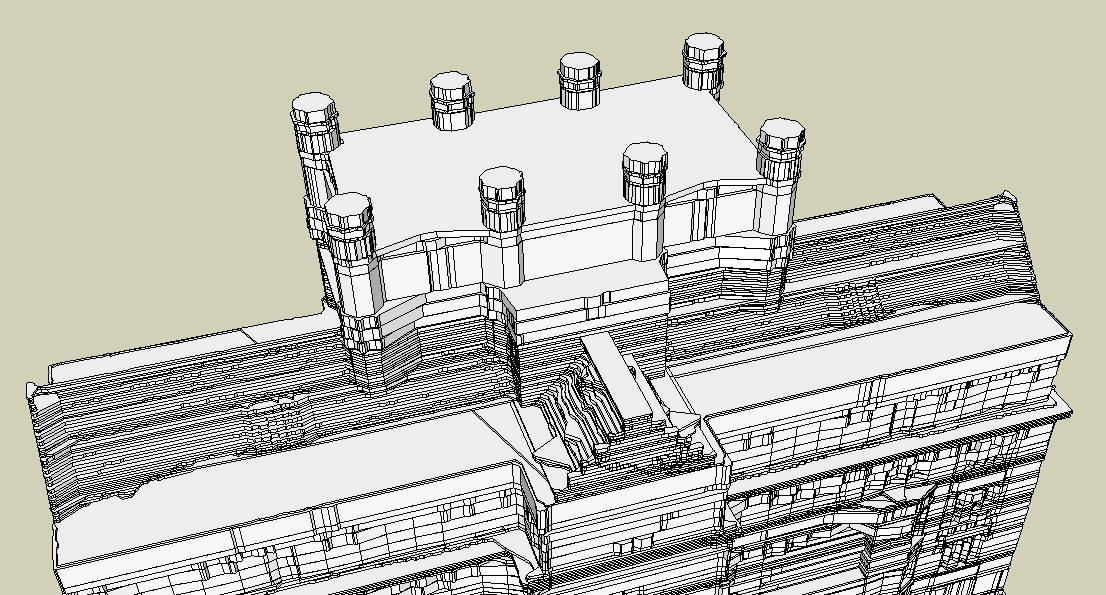
\includegraphics[width=0.35\textwidth]{extrude_1.png} \\
(a) \\
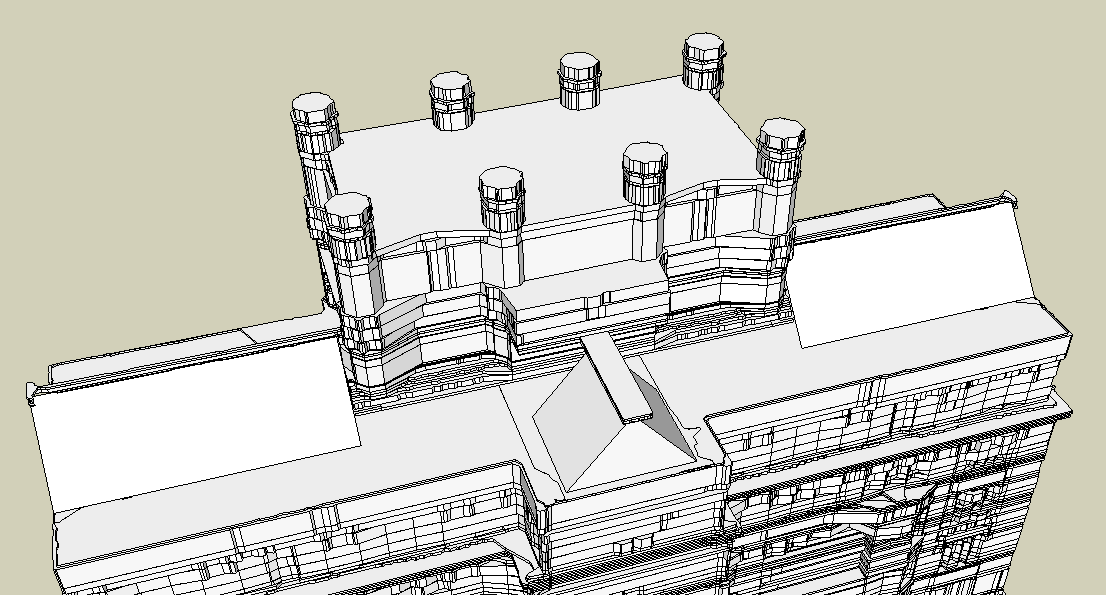
\includegraphics[width=0.35\textwidth]{extrude_2.png} \\
(b)
\end{tabular}
\end{center}
\caption{The top view of the 3D building shown (a) without tapered structures
and (b) with tapered structures.}
\label{fig:DXF_top}
\end{figure}

In addition to the extrusion operation, we can further improve the model
and reduce the model size by observing that part of the keyslice images
belong to the same tapered structure, as demonstrated in \Fig{DXF_top}.
\Figa{DXF_top} shows the roof structure
of the reconstructed model based on a keyslice image extrusion operation with
almost half of the keyslice images dedicated to the structure.
After inferring the tapered structure, \Figb{DXF_top} shows the improvement
of the modeling, which is much smoother than the previous model.
In addition, the keyslices needed to represent the building, and its
associated storage, are reduced almost in half.

The difficulty in inferring tapered structures is tied to the complexity of
the building structure itself.
Let's assume that the height range for the roof structure is
$H_R = [H_{lo}, H_{hi}]$.
If this is the only existing structure between $H_R$, it is simple and
straight-forward to detect and infer this part.
However, for some complicated structures, such as a mixed layout
of tapered and extruded structures, as depicted in \Fig{taper_seg},
some special treatment is needed to obtain the desired results.
Our approach is based on the divide-and-conquer strategy:
the whole structure $\boldsymbol{U}$ is segmented into independent
sub-structure units, $U_0, U_1, \ldots, U_N$.
Any sub-structure unit $U_i$ is constrained to contain a unique structure,
i.e., either a tapered or an extruded one.
Once each unit $U_i$ is inferred, the whole structure can be modeled by a
union operation of these sub-structures, i.e.,
$\boldsymbol{U} = \bigcup{U_i\{ i = 1,\ldots,N\}}$.
Before segmentation, the potential height ranges $H_R$ containing the tapered
structures must be computed.
This can be done by checking the frequency of the keyslice images.
The structure containing tapered sub-structures will show a wide and uniform
distribution of keyslice images.
This is a very useful clue for $H_R$ detection.

\begin{figure}[htbp]
\begin{center}
\begin{tabular}{cc}
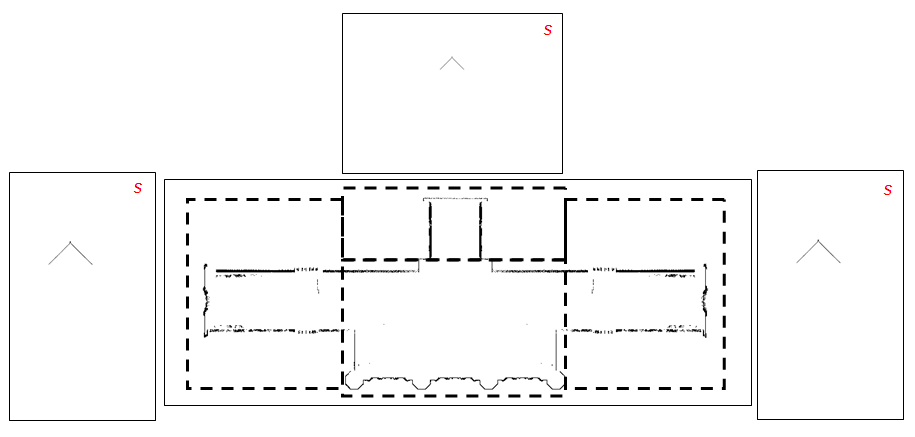
\includegraphics[width=0.45\textwidth]{extrude_3.png} \\
\end{tabular}
\end{center}
\caption{The top view of the 3D building. }
\label{fig:taper_seg}
\end{figure}

Once the potential height ranges $H_R$ is obtained, the next step is to
segment the whole structure $\boldsymbol{U}$ between $H_R$ into sub-structures,
$U_i, \; i = 0,\ldots,N$.
This is again done by applying the similarity measurement to sliced images
from orthogonal directions.
As before, the 3D data points inside the range of $H_R$ are projected
along both left-right ($X$ axis) and face-inside ($Z$ axis) directions.
Then, the keyslice detection is carried out based on the Hausdorff distance
similarity measurement for both directions.
These keyslices will segment the structure in $H_R$ into subunits of
$U_0, U_1, \ldots, U_N$.

For each subunit $U_i$, we must determine whether it represents an extruded or
a tapered structure.
This is done by checking in keyslice image $I_k$ of $U_i$ whether there exists
a pattern where two lines intersect with some appropriate angle.
If such a pattern exists in $I_k$, such as the images marked with red $s$ in
\Fig{taper_seg}, the unit $U_i$ is considered to be a tapered sub-structure unit.
Otherwise, $U_i$ is treated as an extruded sub-structure unit.
If $U_i$ is an extruded unit, its contours from the $y-$ axis are vectorized
and is ready for the union operation to obtain $\boldsymbol{U}$.
On the other hand, if $U_i$ is a tapered unit, the bottom and top position
have to be computed so that it can be reconstructed.
To do this, all line segments $\boldsymbol{L}$ in $U_i$ are computed using
the Hough Transform and the intersection point $P_0$ of $\boldsymbol{L}$
indicates the top position of the tapered unit.
The other end points $P_i$ of $\boldsymbol{L}$ are also computed to infer
the bottom shape and position.

%%%%%%%%%%%%%%%%%%%%%%%%%%%%%%%%
%%%%%%   Experimental Results%%%
%%%%%%%%%%%%%%%%%%%%%%%%%%%%%%%%
\section{Experimental Results}
\label{sec:IR_OUT}

The results of the extrusion and tapered structures computation,
together with keyslice image vectorization, are stored in the 2D
image coordinate system. To generate the final 3D model, these
data need to be transformed back into the 3D world coordinate system.
Let $P(x,y)$ be a point in the 2D image coordinate system, and let $P'(x,y,z)$
be the 3D world coordinate of $P$, where $y$ is the depth coordinate.
For all points in the same contour, the points lie in the same plane and
hence have the same value of $y$.
The equation for transforming $P$ back to $P'$ is a reverse transformation
of $\boldsymbol{T_0}$ in \Eq{image_slicing}:
\begin{equation}
[\,x^{3D},\; y^{3D},\; z^{3D}\,]^T = [\,\eta\cdot x^{2D} + X_{MIN},\; \zeta + Y_{MIN},\; \eta\cdot z^{2D} + Z_{MIN}\,]^T
\label{eq:ir2dxf}
\end{equation}
where $\eta=1/\omega$ and $\zeta=\kappa\cdot\delta$. Here, $\kappa$ is the
index of the 2D slice and $\delta$ is the height of a slab, as described
in \Sec{image_slicing}.
\Figd{IR_2_DXF} shows an exterior 3D model generated by the above
transformation.

\begin{figure*}[htbp]
\begin{center}
\begin{tabular}{cc}
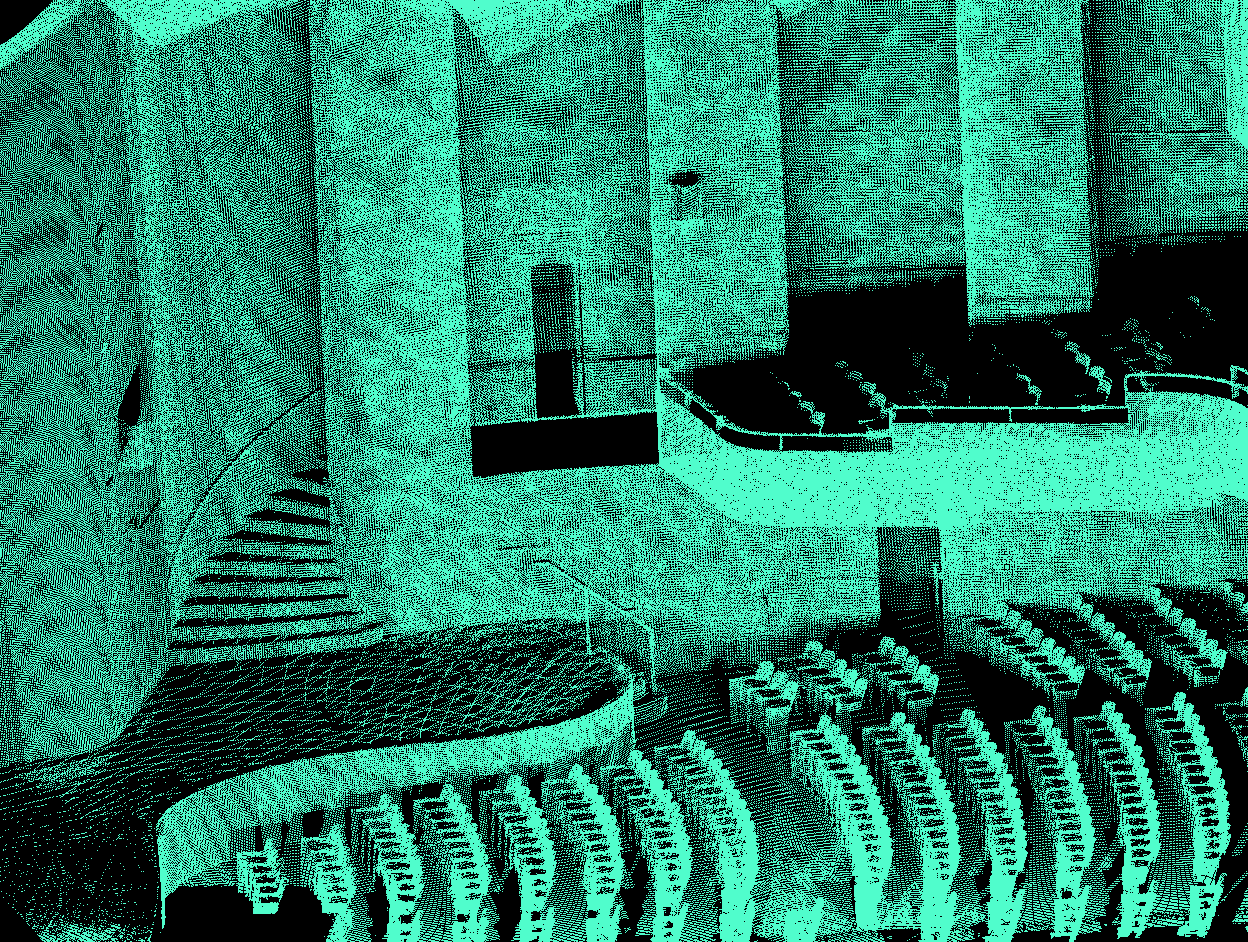
\includegraphics[width=2.5in]{range_crop.png} &
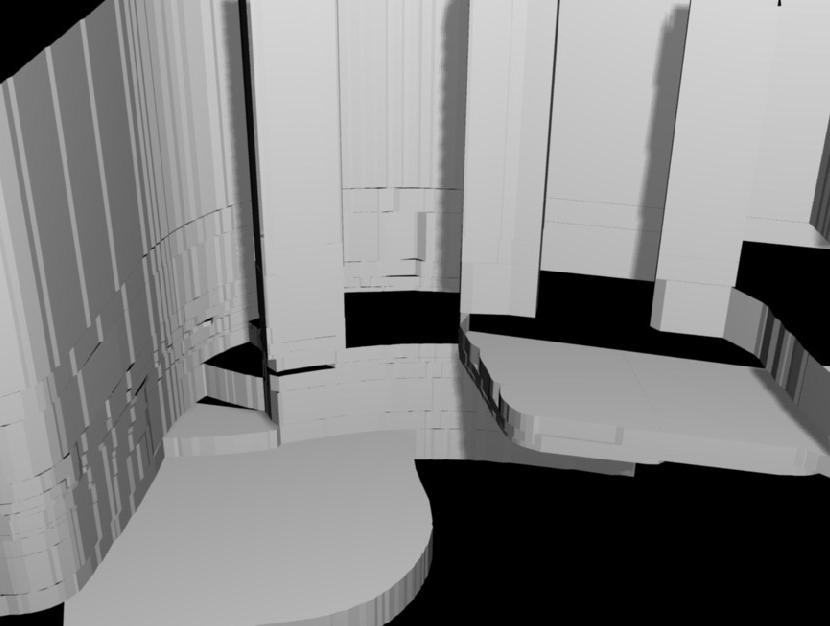
\includegraphics[width=2.5in]{HunterTheatreShaded.jpg} \\
(a) & (b)
\end{tabular}
\end{center}
\caption{The model of an interior scan. (a) Point cloud data and the
(b) reconstructed lightweight 3D model.}
\label{fig:IN}
\end{figure*}

In addition to exterior models, we have also applied the lightweight
reconstruction algorithm to the range data of interior scans.
The snapshot of an interior scan is shown in \Figa{IN}
and its reconstructed 3D model is shown in \Figb{IN}.
This model is primarily reconstructed using the extrusion unit
upon the main structures of the interior.
The chairs and some other fine details were manually culled.
Please note that the model generated in \Figb{IN} is of low resolution.
Any lost detail may be recaptured by using a smaller threshold $\tau_d$
to obtain higher resolution models.

To measure the error of a reconstructed 3D model, we first transform it
to the 3D point cloud coordinate system.
The error $E$ is measured as the distance between the 3D points in the cloud
to their closest planes in the reconstructed model $M$:
\begin{equation}
E = \frac{1}{|X|}\sum_{x\in{X}}{d^2(x, M)}
\label{eq:em}
\end{equation}
where $X$ is the set of 3D points in the point cloud, and distance
$d(x, M) = \text{min}_{p \in M}\lVert x - p \lVert$ is the minimum
Euclidean distance from a 3D point $x$ to its closest face $p$ of $M$.

\begin{figure} [htbp]
\begin{center}
\begin{tabular}{cc}
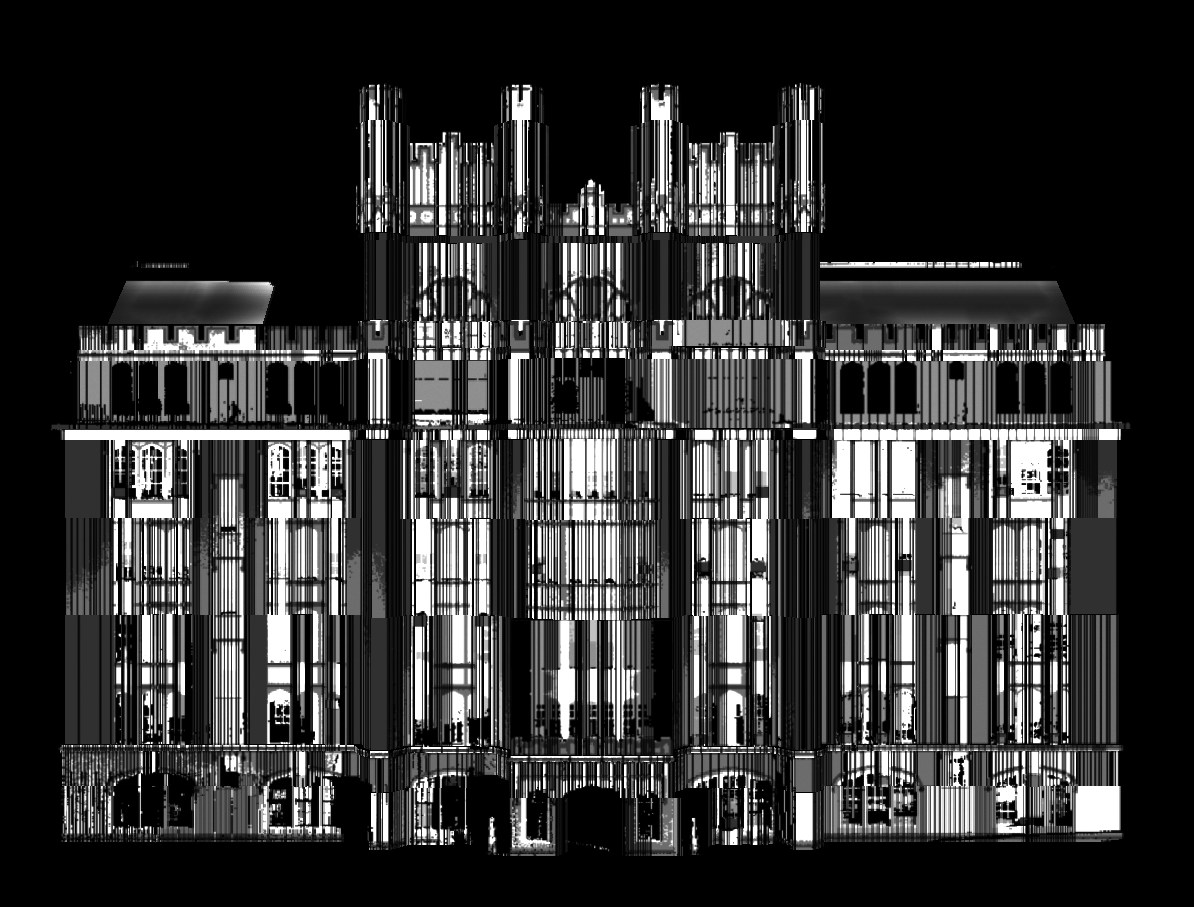
\includegraphics[width=0.2\textwidth]{error_1000_32_4.png} &
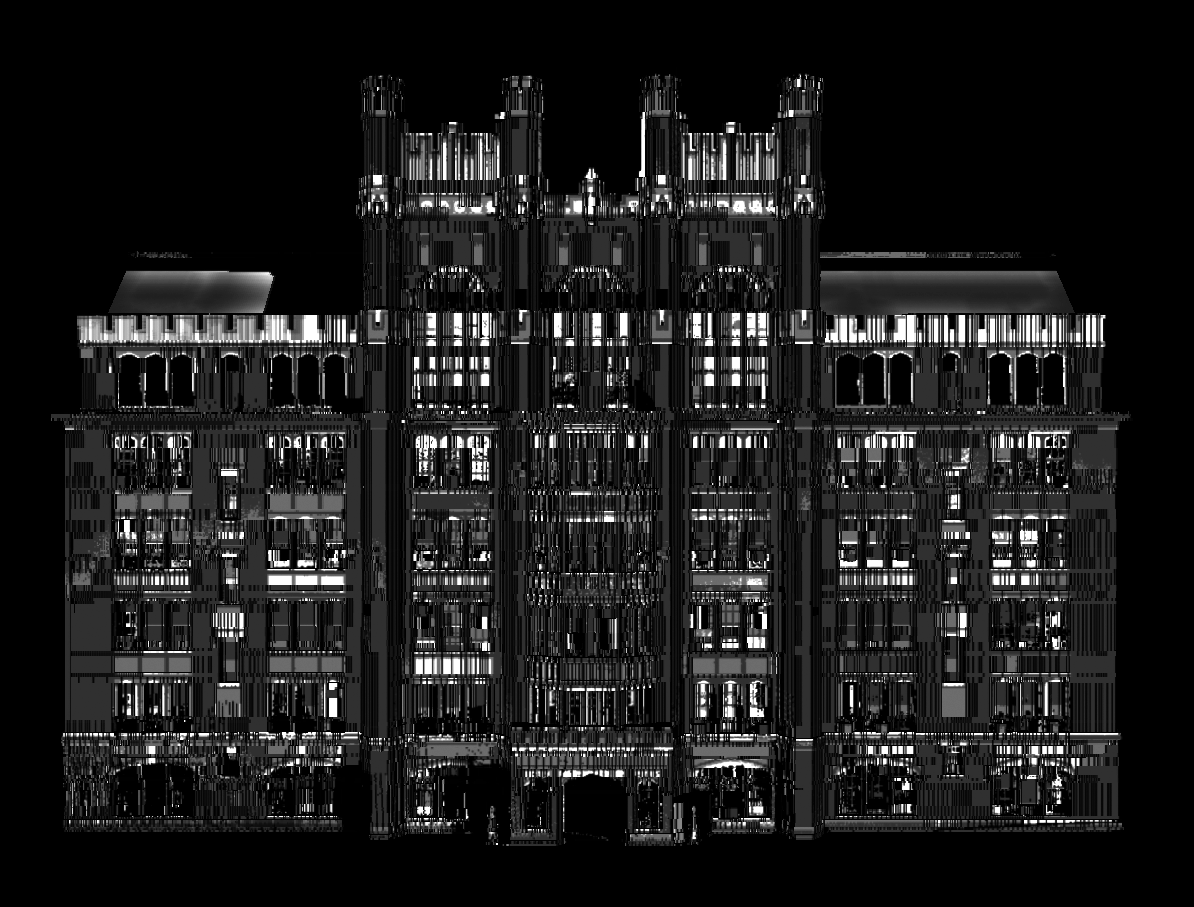
\includegraphics[width=0.2\textwidth]{error_1000_4_1.png} \\
(a) & (b)
\end{tabular}
\end{center}
\caption{The deviation map of the 3D point cloud. (a) The result with $\tau_r$ = 4 and $\tau_d$ = 32.
(b) The result with $\tau_r$ = 1 and $\tau_d$ = 4. }
\label{fig:EM}
\end{figure}

To visualize the error between real 3D data and the inferred model,
we generate deviation map images.
Two such images are shown in \Fig{EM} for the point cloud data in
\Figb{IR_2_DXF}.
The deviation maps are constructed as follows.
For each face $p$ of $M$, a corresponding texture image is computed.
The intensity of each pixel in the texture image is determined by the error
of the corresponding 3D points computed by \Eq{em}.
The accuracy of the reconstructed model is controlled by Hausdorff distance
threshold $\tau_d$ and BPA refinement radius $\tau_r$.
Threshold $\tau_d$ determines the accuracy of keyslice detection and $\tau_r$
determines the accuracy of boundary vectorization.

\Tbl{em} lists the relationship among the $\tau_d$, errors,
number of faces, and model size for the input data in \Figb{IR_2_DXF}.
The units for $\tau_d$ and error is in pixels and millimeters, respectively.
The size of the original point cloud for the 3D building is more than 700 MB.
From the table, one can see that even for the most accurate model, the size
is dramatically reduced compared with the original 3D point cloud data.
This is a desirable property for web-based applications (\Figd{IR_2_DXF}).
The low resolution ($\tau_d = 64$) and high resolution ($\tau_d = 4$) models
were generated in 15 and 120 minutes, respectively,
on a laptop PC running an Intel Core 2 T7200 CPU at 2.0 GHz with 2.0 GB RAM.
Future work includes the optimization of the BPA vectorization module since
it consumes approximately 70\% of the computation time.

\setlength{\tabcolsep}{4pt}
\begin{table}[hbtp]
\begin{center}
\begin{tabular}[t]{||c||c|c|c||}
\hline
$\tau_{d} $(pixel) & Error (mm)& \# of faces & Size (KB) \\ \hline \hline
64 & 0.658 & 1471  & 15  \\ \hline
32 & 0.294 & 3284  & 32  \\ \hline
16 & 0.141 & 8574  & 86  \\ \hline
8  & 0.131 & 13955 & 137 \\ \hline
4  & 0.094 & 27214 & 261 \\ \hline
2  & 0.088 & 31331 & 335 \\ \hline
1  & 0.083 & 32187 & 337 \\ \hline
\end{tabular}
\end{center}
\caption{Error measurements for reconstruction of \Figb{IR_2_DXF} using
Hausdorff distance threshold $\tau_d$ and BPA radius threshold $\tau_r = 4$.}
\label{tbl:em}
\end{table}
\setlength{\tabcolsep}{1.4pt}

\section{Model Comparison}

Although models generated by 3D BPA are of high resolution, they usually
require excessive storage capacity.
The model in \Fig{TH_BPA}, for example, needs almost 400 MB of storage,
which prevents this solution from being applied to web-based applications.
One way to improve matters is to apply some approximation/decimation
technique to reduce the space required by these models.

The holes in the 3D BPA model in \Fig{TH_BPA} are present in the
original dataset.
They are due to the fact that the laser never reflected back to
the scanner after penetrating the glass windows.
The 3D BPA method is deficient in filling these holes.
We counter this problem by first applying a symmetry-based hole filling
algorithm on the 2D slices to create enhanced slices that are processed
by an adaptive 2D BPA method to fill gaps.
Finally, an extrusion operation is applied to create a watertight 3D model.

\begin{figure}[htbp]
\begin{center}
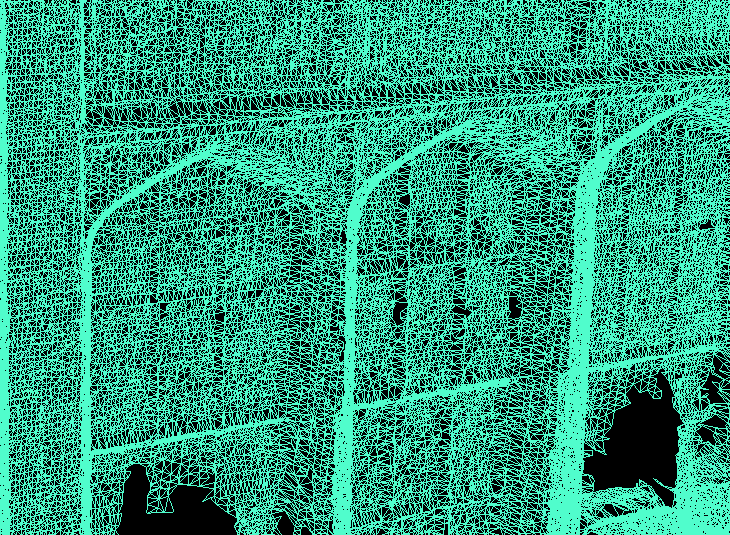
\includegraphics[width=2.5in]{BPA_TH.png}
\end{center}
\caption{Dense triangulated BPA mesh cropped from \Figb{IR_2_DXF}.}
\label{fig:TH_BPA}
\end{figure}

Among all mesh reduction techniques, {\it qslim} is one of the most
sophisticated and efficient algorithms.
We carried out a comparison between models generated by our proposed
method and those approximated by {\it qslim}.
The comparisons were conducted on models sharing the same number of faces.
It is worth noting that {\it qslim} ran out of memory on the 3D model data
generated by BPA in \Fig{TH_BPA}.
In order to reduce the size of the model for {\it qslim} to work, we had
to either downsample the 3D model generated by BPA or split it into
sub-models which can be handled by {\it qslim}.

\begin{figure}[htbp]
\begin{center}
\begin{tabular}{cc}
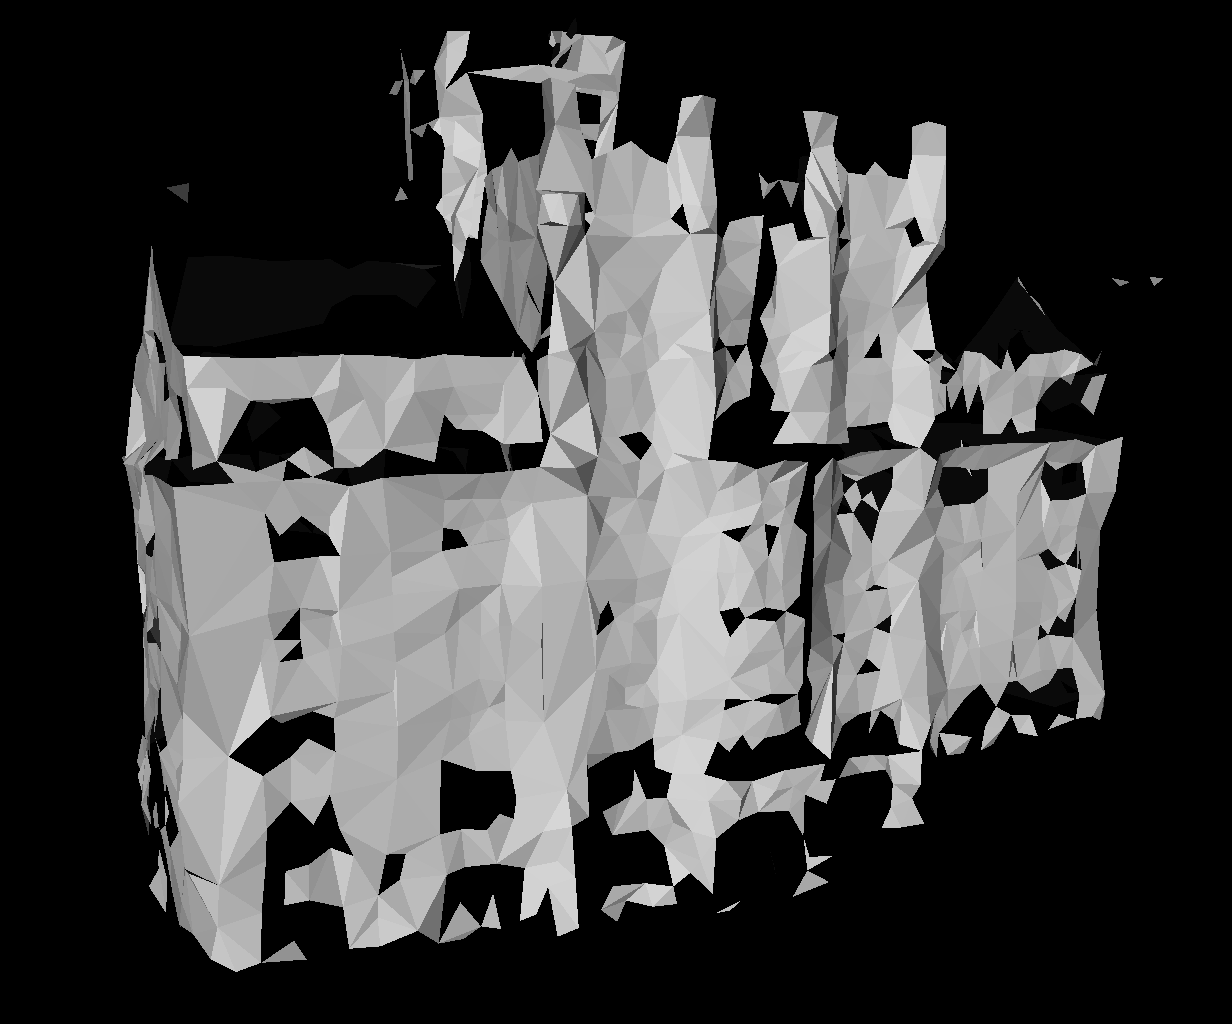
\includegraphics[width=0.2\textwidth]{comp_32_2_qslim.png} &
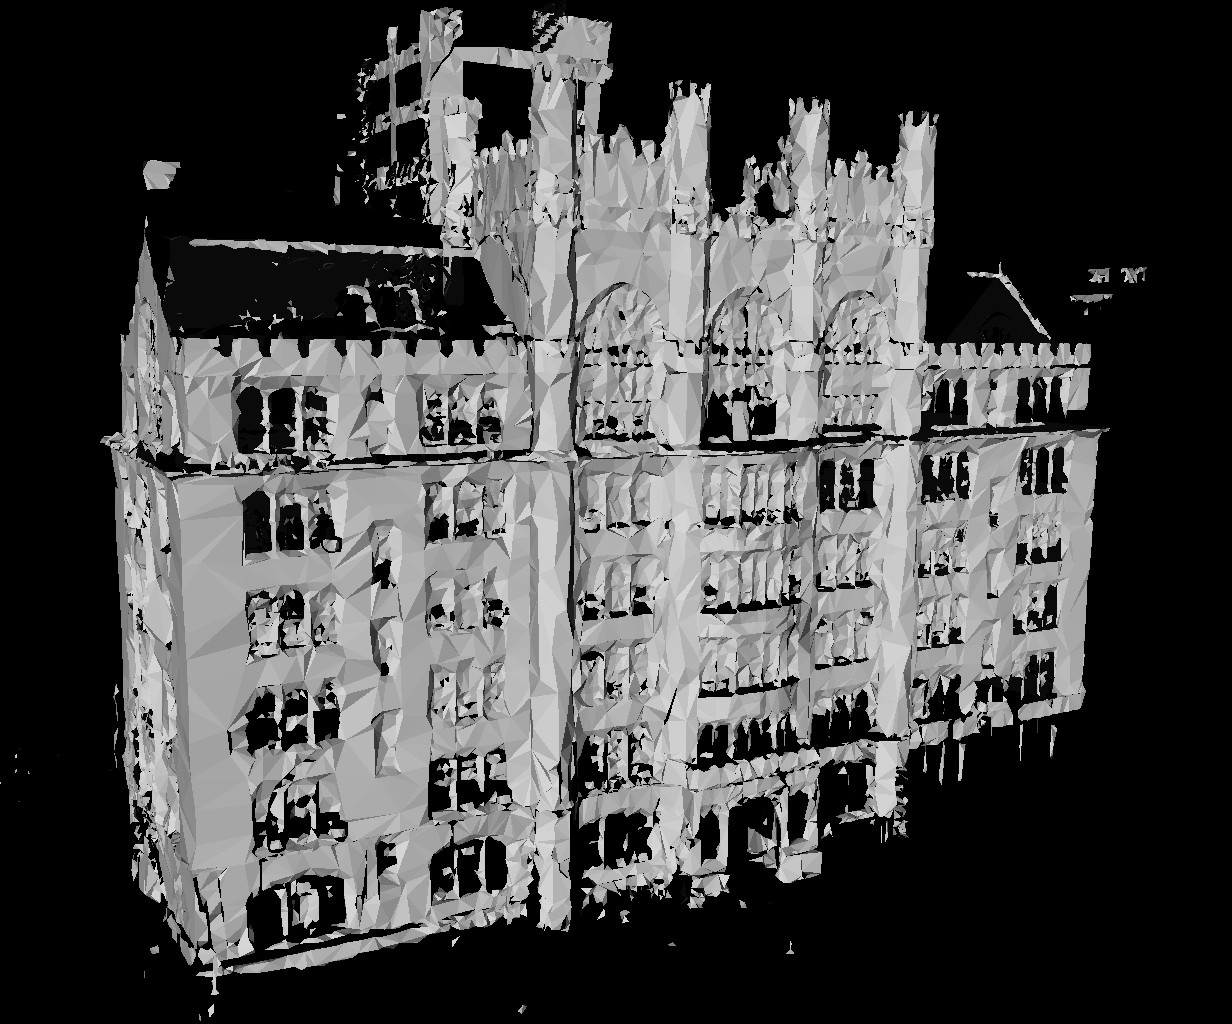
\includegraphics[width=0.2\textwidth]{comp_4_2_qslim.png} \\
(a) & (b) \\
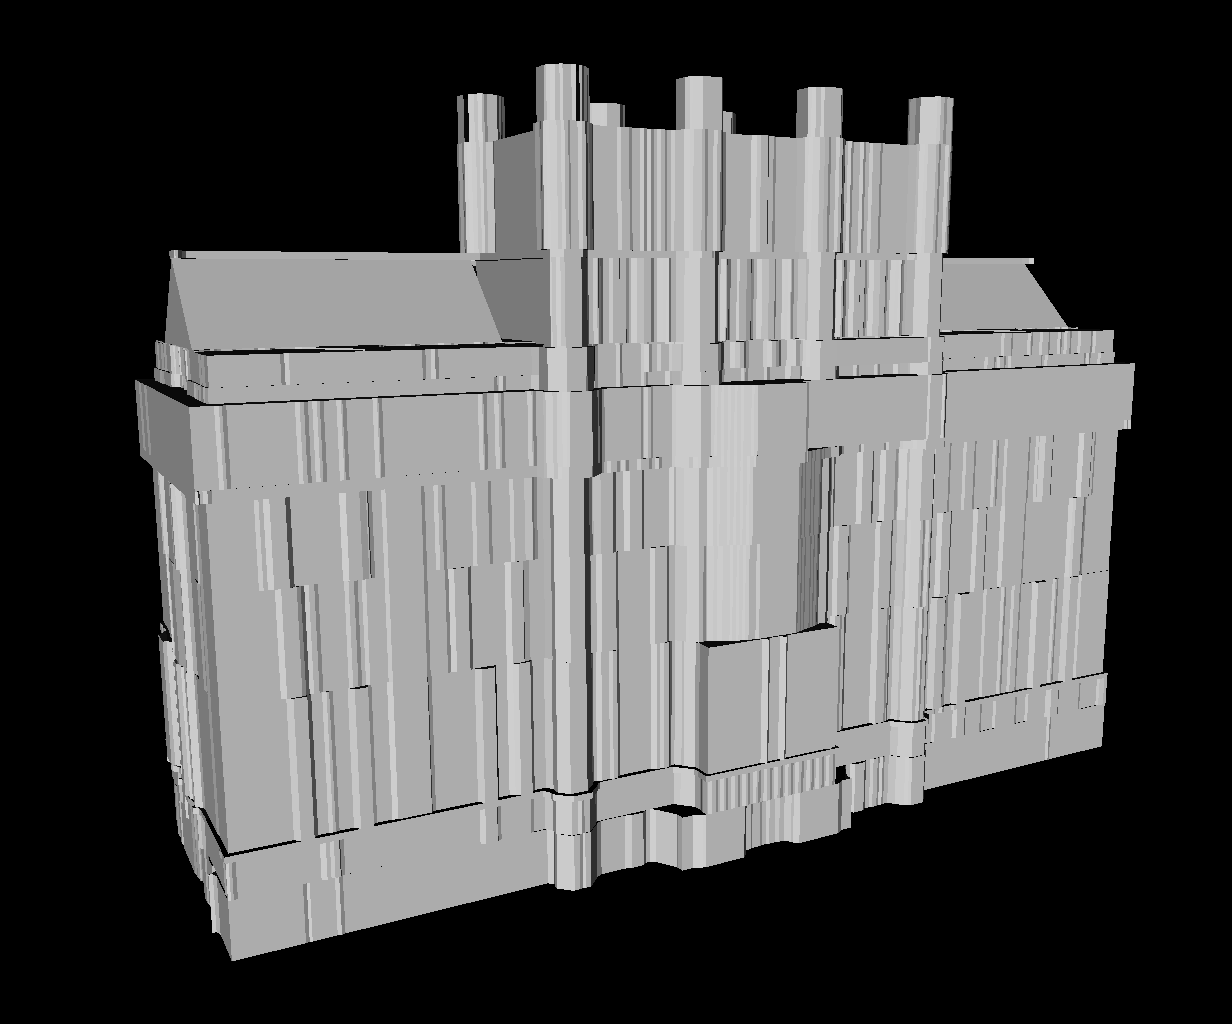
\includegraphics[width=0.2\textwidth]{comp_32_2.png} &
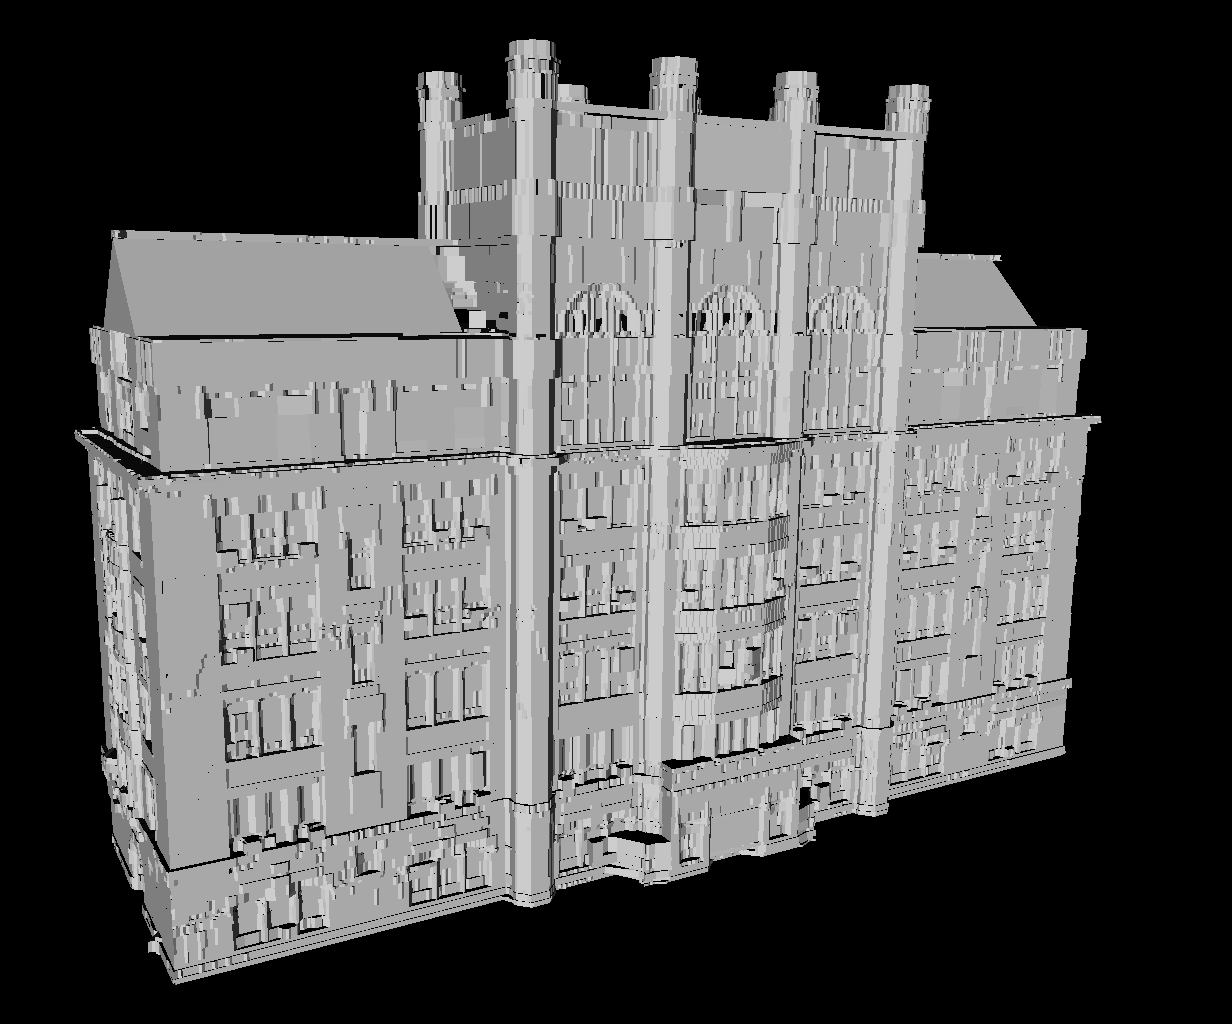
\includegraphics[width=0.2\textwidth]{comp_4_2.png} \\
(c) & (d)
\end{tabular}
\end{center}
\caption{
Models generated by {\it qslim} having (a) 2,000 and (b) 32,000 faces.
Models generated by our approach having (c) 2,000 and (d) 32,000 faces.}
\label{fig:TH_comp}
\end{figure}

\Figa{TH_comp} and \Figc{TH_comp} respectively depict the models generated
by {\it qslim} and our proposed method with approximately 2,000 faces each.
Higher resolution models with roughly 32,000 faces each are shown in
\Figb{TH_comp} and \Figd{TH_comp}.
Notice that the models approximated by {\it qslim} are inferior since they
do not preserve the sharpness of the original model and are replete with
holes. Our symmetry detector and extrusion operation guarantees no holes.

%%%%%%%%%%%%%%%%%%%%%%%%%%%%%%%%
%%%%%%   Conclusion and Future Work%%%
%%%%%%%%%%%%%%%%%%%%%%%%%%%%%%%%
\section{Conclusion and Future Work}

This paper has presented an efficient algorithm for lightweight 3D modeling
of urban buildings from range data.
Our work is based on the observation that buildings can be viewed as the
combination of two basic components: extrusion and tapering.
The range data is partitioned into volumetric slabs whose 3D points are
projected onto a series of uniform cross-sectional planes.
The points in those planes are vectorized using an adaptive BPA algorithm
to form a set of polygonal contour slices.
Prominent keyslices are extracted from this set.
Applying extrusion to these keyslices forms lightweight 3D models.
Experimental results on both exterior and interior urban building datasets
have been presented to validate the proposed approach.

We achieve further geometry compression by detecting a series of
slices that coincide with a taper operation.
In the current work, we demonstrate how to infer the taper-to-line
geometry structure.
In future work we will extend this to include the taper-to-point geometry
structure, which appears frequently in Gothic architecture (e.g., churches).
A nice characteristic of this structure is that the image slices will converge
to a point, which is a good inference cue.

Additional future work is to investigate the modeling of the ``follow-me''
geometry structure.
This is a more complicated geometry structure featured in Google SketchUp
that exists when the model can be reconstructed by moving a cross-sectional
unit along a curve trajectory.
We will track the slices to obtain the curve trajectory.
Finally, we will optimize the performance of the BPA vectorization module,
which consumes the bulk of the computation time.

\bibliographystyle{acmsiggraph}
\bibliography{sigASIA09}

\end{document}
